\documentclass[10pt]{article}
% \usepackage[margin=1in]{geometry}
% \newcommand\hmmax{0}
% \newcommand\bmmax{0}
% % % Fonts% %
\usepackage[T1]{fontenc}
   % \usepackage{textcomp}
   % \usepackage{newtxtext}
   % \renewcommand\rmdefault{Pym} %\usepackage{mathptmx} %\usepackage{times}
\usepackage[complete, subscriptcorrection, slantedGreek, mtpfrak, mtpbb, mtpcal]{mtpro2}
   \usepackage{bm}% Access to bold math symbols
   % \usepackage[onlytext]{MinionPro}
   \usepackage[no-math]{fontspec}
   \defaultfontfeatures{Ligatures=TeX,Numbers={Proportional}}
   \newfontfeature{Microtype}{protrusion=default;expansion=default;}
   \setmainfont[Ligatures=TeX]{Source Serif Pro}
   \setsansfont[Microtype,Scale=MatchLowercase,Ligatures=TeX,BoldFont={* Semibold}]{Source Sans Pro}
   \setmonofont[Scale=0.8]{Atlas Typewriter}
   % \usepackage{selnolig}% For suppressing certain typographic ligatures automatically
   \usepackage{microtype}
% % % % % % %
\usepackage{amsthm}         % (in part) For the defined environments
\usepackage{mathtools}      % Improves  on amsmaths/mtpro2
\usepackage{amsthm}         % (in part) For the defined environments
\usepackage{mathtools}      % Improves on amsmaths/mtpro2
\usepackage{xfrac}

% % % The bibliography % % %
\usepackage[backend=biber,
  style=authoryear-comp,
  bibstyle=authoryear,
  citestyle=authoryear-comp,
  uniquename=false,%allinit,
  % giveninits=true,
  backref=false,
  hyperref=true,
  url=false,
  isbn=false,
  useprefix=true,
  ]{biblatex}
\DeclareFieldFormat{postnote}{#1}
\DeclareFieldFormat{multipostnote}{#1}
% \setlength\bibitemsep{1.5\itemsep}
\newcommand{\noopsort}[1]{}
\addbibresource{Thesis.bib}

% % % % % % % % % % % % % % %

\usepackage[inline]{enumitem}
\setlist[itemize]{noitemsep}
\setlist[description]{style=unboxed,leftmargin=\parindent,labelindent=\parindent,font=\normalfont\space}
\setlist[enumerate]{noitemsep}

% % % Misc packages % % %
\usepackage{setspace}
% \usepackage{refcheck} % Can be used for checking references
% \usepackage{lineno}   % For line numbers
% \usepackage{hyphenat} % For \hyp{} hyphenation command, and general hyphenation stuff
\usepackage{subcaption}
% % % % % % % % % % % % %

% % % Red Math % % %
\usepackage[usenames, dvipsnames]{xcolor}
% \usepackage{everysel}
% \EverySelectfont{\color{black}}
% \everymath{\color{red}}
% \everydisplay{\color{black}}
\definecolor{fuchsia}{HTML}{FE4164}%Neon Fuchsia %{F535AA}%Neon Pink
% % % % % % % % % %

\usepackage{pifont}
\newcommand{\hand}{\ding{43}}
\usepackage{array}


\usepackage{multirow}
\usepackage{adjustbox}

\usepackage{titlesec}

\makeatletter
\newcommand{\clabel}[2]{%
   \protected@write \@auxout {}{\string \newlabel {#1}{{#2}{\thepage}{#2}{#1}{}} }%
   \hypertarget{#1}{#2}
}
\makeatother

\usepackage{multicol}

\setcounter{secnumdepth}{4}
\setcounter{tocdepth}{4}

\usepackage{tikz}
\usetikzlibrary{bending,arrows,positioning,calc}
\usepackage{tikz-qtree} %for simple tree syntax
% \usepgflibrary{arrows} %for arrow endings
% \usetikzlibrary{positioning,shapes.multipart} %for structured nodes
\usetikzlibrary{tikzmark}
\usetikzlibrary{patterns}


\usepackage{graphicx} % for images (png/jpeg etc.)
\usepackage{caption} % for \caption* command


\usepackage{tabularx}

\usepackage{bussalt}

\usepackage{Oblique} % Custom package for oblique commands
\usepackage{CustomTheorems}

\usepackage{svg}
\usepackage[off]{svg-extract}
\svgsetup{clean=true}



\usepackage{dashrule}

\newcommand{\hozline}[0]{%
  \noindent\hdashrule[0.5ex][c]{\textwidth}{.1pt}{}
  %\vspace{-10pt}
  % \noindent\rule{\textwidth}{.1pt}
}

\newcommand{\hozlinedash}[0]{%
  \noindent\hdashrule[0.5ex][c]{\textwidth}{.1pt}{2.5pt}
  %\vspace{-10pt}
}

\usepackage{contour}
% \usepackage{pdfrender}

\usepackage{extarrows}

\usepackage[hidelinks,breaklinks]{hyperref}

\title{Means-end reasoning and means-end relations}
\author{Ben Sparkes}
% \date{ }


\begin{document}

Literature on reasons and reasoning.
Data point.
Grey area.

Started as a puzzle.

Fits into the literature\dots
Some views permits, but are non-committal.
Other view conjecture.
Others provide insight.

If you are interested in ideal rationality, then this kind of case can be rejected.

If, however, you are interested in less-than-ideal rationality, then perhaps these types of cases are of interest.




Supplement to the literature.
Kind of case that pushes on various parts, but overlooked.
Case doesn't depend on literature, but can learn something.

Hum, could this be about how the ideal relates to actual agents?

So, something of a grey area.
The phenomena can be understood on various accounts.
It's not clear what is to be said.

Literature.
Distinct kinds of rational pressure.
Push in different directions.

Here, cooperation.
Agent's attitude toward a proposition is the result of two kinds of pressure which cannot be separated.

Here, argue that the agent continues to recognise pressure based on attitudes that the agent has, but is unaware of how the pressure is generated.
Dynamics of rationality, how to understand agents.
Cases in which an agent will respond to (primarily) attitude based pressure on the basis of (primarily) evidence based pressure.

General type of case.
Framed in terms of epistemic attitudes, but key is that the relevant property does not depend on reasoning.




The puzzle here is that there's something that the agent hasn't done, and not that there's any kind of conflict.
This, I think, is the distinguishing feature of the case.
On the one hand, I'm not all that concerned with what's going on, and all I really want is for the pressure to exist.
However, focusing on the idea that there is pressure is a good way to get this without arguing for it directly.
Though, better yet, it provides an argument for it being the case that pressure exists.

If I'm right about pressure, then there's no issue of trust.

The core idea is that the agent recognises that if they were to reason, then they would settle on \(\phi\) without any additional information.

This differentiates the case from reflection principles.
It's also not identical to the issue of whether evidence of evidence is evidence.
\begin{itemize}
\item This is a somewhat subtle point, but the idea is that the focus is on reasoning from the commitments that you have is not identical to responding to evidence.
\item That's because, in short, it's the attitudes that are doing the work, and not necessarily the evidence.
\item The idea is that there can be evidence for evidence of \(\phi\) but also evidence that \(\phi\) is false.
  Case in which the agent says that they were convinced that they found a winning strategy but were mistaken.
  Now what?
  It seems the agent should be confident that they would make a mistake if they were to reason.
  This happens.
  The test is really hard, and I was convinced that a certain answer was correct but it wasn't.
  The agent then takes the test, and gets the answer wrong.
  This is kind of the structure of trick questions, 
\end{itemize}
Hum, well, this suggests I need to do a little more, as it's not clear that attitudes aren't evidence.
I'd need a case in which the agent recognises that they've been misled about the evidence, \dots
So, back to detectives in the spirit of Christensen.
Here, detective is consulting the companion, and says that we were wrong in thinking that the evidence pointed to someone being the culprit.
And, this is because of a bad prior.
The companion is confident that they have the same prior, and so they think that they would mistakenly reason to the someone being the culprit.
And, the problem is that their attitudes support this, though they do not take these to be evidence.
So, the companion is not applying evidence of evidence is evidence, or coherent requirements, etc.
And, it seems the fix is not \emph{only} to believe that the someone is not the culprit.
For, if the companion reasons from their attitudes they will go wrong.
For sure, the detective can make a point that the evidence was fine and that some prior was problematic.

These attitudes are linked, and there's dynamics due to the links between the attitudes, and we view these links as present even if they are not recognised in the moment.
This is sort of a Harman point, in the sense that some things are left to reasoning to avoid clutter.

\section{Outline}
\label{sec:outline}

\begin{enumerate}
\item Scenario
\item Reference problem
\item Testimony
\item Framework
\item Attitudes
\item Criminality
  \begin{itemize}
  \item Different kind of bounded rationality.
  \item Unlike that of \citeauthor{Simon:1957aa}, as this doesn't look to tractable problems.
  \end{itemize}
\end{enumerate}

\section{Ideas}
\label{sec:ideas}

\begin{itemize}
\item Appeal to the distinction between propositional and doxastic justification to motivate the two pressures on an agent.
\item Explain issue in terms of this.
\item This is related to the distinction between justification and coherence, etc.
  However, it seems as though coherence is a way of capturing the requirements related to doxastic justification.
\item Important to note that nothing really goes wrong, so it's not quite the same as wrongs kind of reasons cases.
\item Similarly to the wrong kind of reasons, there's no deviant causal chain here, though there are similarities.
\item Note that this gets difficult in cases of testimony.
\end{itemize}


\section{Scenario}
\label{sec:scenario}

An agent and a companion are playing chess together.
Specifically, an agent and a companion are playing arbitrary many games of chess together.
Both the agent and the companion have a clear view of the board, and both have a comprehensive understanding of the rules of chess.
The board mediates all interaction between the agent and the companion with one exception.
The exception is that the agent and companion are allowed to ask each other whether the agent has a winning strategy and whether the companion has a winning strategy, and the other player is allowed to respond with either `yes', `no', or `maybe'.

The agent is looking at the board, is yet to find a move that does not seem to give their companion an advantage, but is considering a few moves do not (to the agent) clearly lead to a loss.
The agent decides to ask their companion whether the companion has a winning strategy, and the companion responds `yes'.

Should the agent believe that the companion has a winning strategy?

The previous interaction between the agent and the companion has show that whenever the agent has settled on an answer the companion has settled on the same answer.
And, whenever the agent or companion has answered `yes' to having a winning strategy the respective player has won the game for which the question was asked.
There may have been multiple occasions on which a winning strategy existed but was not discovered by either player.

So, whenever the question of whether a winning strategy exists for a player has be answered `yes' by either the agent of the companion, the agent had settled on `yes' as an answer to the same question independently of the companions answer to the question (by identifying a winning strategy for the player) and sometimes a winning strategy was then used by the player for which the question was raised while other times the player without the winning strategy resigned the game.

Unlike previous games, the agent has asked the companion whether the companion has a winning strategy without settling on an answer to whether the companion has a winning strategy, and the companion has answered `yes'.

It seems likely that if the companion answers `yes' to whether a winning strategy for a player exists, then a winning strategy does exist for that player.
For, every time the companion has answered `yes', a winning strategy has been employed by that player.

Is the current problem similar to previous problems?

Have the class of questions, and looking at the confidence that there is a winning strategy given the companion has answered `yes' to the question of whether there is a winning strategy.
Agent has built up some degree of confidence, and one can wonder whether the agent's confidence is representative of the larger class.
Perhaps the games that have been played are just those for which the companion answers `yes' only if (but not necessarily if) a winning strategy exists.
\begin{itemize}
\item General scepticism about inductive reasoning.
\item Not the issue I'm interested in.
\end{itemize}

Instead, reference class.
Agent doesn't have any information about the reliability of the companion when the agent has not independently reasoned to a winning strategy.

If the agent could reason to a winning strategy, then the agent can be confident.
If the agent cannot, then there's some difference.

There's background information here, and it makes a difference.

Here, something about the agent and companion answering more or less independently of one another.

At some point while contemplating the next move the agent and companion settle on an answer of `yes', `no', or `maybe' to whether the agent has a winning strategy and whether the companion has a winning strategy.
So, whether or not the agent has settled on an answer to whether the companion has a winning strategy is not related to whether the agent has \emph{reasoned} to a winning strategy, but whether or not the agent is \emph{able to reason} to a winning strategy.
Hence, while there may be a difference between the agent having settled on an answer and the agent being able to settle on an answer, it is reasonable for the agent not to consider this difference relevant.

Whether the agent is able to reason to a winning strategy does make a difference.
For, there have been occasions on which the agent and the companion resigned games after the agent has reasoned to a winning strategy.

The agent has observed that a certain player always wins once the companion answers `yes' to the question of whether the companion has a winning strategy, but in a non-trivial number of cases the player's victory is due to the agent resigning given their recognition of a winning strategy.

\begin{note}
  Here's the way to push for a higher degree of confidence.
\end{note}

So, there will be a non-trivial difference:
If the agent is able to reason to a winning strategy then the agent should have a greater degree of confidence that a winning strategy for the companion exists.

This difference, given the agent's priors and the number of cases in which the agent resigns may be significantly non-trivial.

\begin{note}
  The point here is that whether or not the agent is able to reason matters to the agent's confidence, and in a non-trivial way.
\end{note}

Should the agent be confident that they are able to reason to a winning strategy?
Plausibly.
Previous cases, and no defeaters.
Really, confident that their ability is matched with the companion.
Put this together with the direction given by the companion.
This is a nice way of putting things, as the agent should not, intuitively, grant that the companion is an expert.

And that's the problem.
It makes a difference, and is reasonable.
The agent's can't appeal simply to the likelihood given the companion's answer without there being a difference that the agent seems to be able to cover.
Confidence won't be that of there being a winning strategy, as the agent must take into account the possibility that they are not able to reason to the winning strategy.
Agent can see the board, has a grasp of the rules, and has matched the companion.

\begin{note}
  This sets up the problem.
  The agent's confidence about their reasoning matters to their confidence about whether the conclusion follows.
\end{note}

The agent's confidence in parity of ability that matters.
With this, the agent tends to greater degree of confidence.

Then, the agent has confidence that they would not otherwise have, but does not have the reason.
The agent has been guided by their ability to reason, but has not done the reasoning.

The companion's answer pushes the agent's confidence around, right.
However, this is just pushing numbers around.

Two things are doing the work.
The companion's answer and parity in ability.
However, given parity in ability, the agent can reason to the companion's answer.
Existence of a winning strategy does not depend on reasoning, but it's identification does.

\subsection{Similar scenario}
\label{sec:similar-scenario}

Do the same thing but with running.
Agent and companion.
Post our results to a website.
I see that there is parity.
Companion Has run a particular route, but agent has not.
Seem the agent should be confident that they can run that route.
Agent should not be confident that they have run the route, but here this is because having run the route depends on the action of the agent.
In the scenario, the existence of a winning strategy does not depend on the action of the agent, it depends on the arrangement of the board and the rules of chess.

In the same way, the agent is not confident that they have reasoned to a winning strategy, as this requires action on the part of the agent.
And, the agent is not confident that they have reasoned to a winning strategy.
It is the agent's confidence that a winning strategy exists that is of interest.

The agent's confidence is based on parity.
Yet, given parity the existence of a winning strategy is quite likely supported by reasoning the agent is able to do.

\begin{note}
  Another is looking up the summary of a book.
\end{note}


\subsection{Analogy}
\label{sec:analogy}

The problem here seems to be similar to a case in which you are confident that a particular piece of a puzzle is fixed to a certain location by looking at the picture that the puzzle depicts.
Even though there's great evidence that you have identified the location of the piece of the puzzle, it follows that if you are correct then there are additional pieces that will connect to the pieces you already have independently of the particular piece, and so you're committed to this, based on what you've done of the puzzle so far.

This is a nice analogy.
Because, it may be that you've made a mistake with the pieces, but the picture still seems right, and so even though the partially completed puzzle is wrong, it's still suggesting that the piece goes in a certain location.



\newpage

\subsection{Intuition}
\label{sec:intuition}

It seems the agent is under pressure from their confidence of parity and their conditional confidence in the correctness of the companion given parity to be confident that there is a winning strategy for the companion.
Yet, it does not seem that this is the only pressure that the agent is under.
For, it seems that the agent is also under pressure to support their confidence that there is a winning strategy by appealing to the state of the board and their grasp of the rules of chess.
That is, if there is a winning strategy, and parity holds, then the agent is able to reason to the winning strategy.

Consider the case that there is not in fact a winning strategy, and the companion is mistaken.
Here it seems that the agent can explain why they were confident that there was a winning strategy, as this was supported by the agent's confidence of parity and their conditional confidence in the correctness of the companion given parity.
However, the agent's explanation does not seem to excuse their mistake, for the agent had the ability to recognise that they did not have support for a winning strategy (given their abilities).

To illustrate with a simpler scenario, assume that both \(P\) and \(P \rightarrow Q\) are well supported by the agent's web of evidence, and the agent is confident that \(P\) and that \(P \rightarrow Q\).
As the agent is confident that \(P\) and that \(P \rightarrow Q\) then the agent should be confident that \(Q\) by well rehearsed arguments regarding coherence between attitudes.
However, suppose in addition the agent observes \(\lnot Q\) and that this does not directly undermine any of the agent's evidence prior to observing \(\lnot Q\).
Then, as the agent has observed \(\lnot Q\) then by well rehearsed arguments relating doxastic confidence to truth it seems the agent should be confident that \(\lnot Q\)
So, coherence continues to require that the agent is confident that \(Q\), if the agent does not adjust their confidence that \(P\) and that \(P \rightarrow Q\), but the agent's observation of \(\lnot Q\) requires that the agent's confidence that \(P\) or that \(P \rightarrow Q\) is revised.
Therefore, as things stand, there is a tension between the what appears to be the case based on observation, and what appears to be the case based on coherence.

Noting the above tension between what appears to be the case based on observation, and what appears to be the case based on coherence is not to deny that there is a clear resolution.
Perhaps the agent should  adjust their confidence so \(Q\) is not required by coherence or perhaps the agent should doubt their observation of \(\lnot Q\) is veridical, more needs to be said to decided the issue.
However, hopefully the potential for these two ways of supporting attitudes toward \((\lnot)Q\) to (appear to) conflict is intuitive.

\textcite{Fogal:2019aa} seems to capture this tension by distinguishing between \emph{substantive rationality} and \emph{structural rationality}.

\begin{description}[font=\bfseries, leftmargin=.75cm, style=nextline]
\item[Substantive rationality] [T]he sense in which it's rational to believe that the sun will rise tomorrow or that grass is green, but irrational to believe that you're smarter than Einstein or that the moon is made of cheese, since the evidence had by nearly everyone—including you—strongly supports both of the former but neither of the latter.\nolinebreak
  \mbox{}\hfill\mbox{(\citeyear[1]{Fogal:2019aa})}
\item[Structural rationality] [T]he sense in which it's rational to believe the obvious consequences of other things you believe and take the means you believe to be required to achieve your ends, while it's irrational to believe something you think is unsupported by the evidence or intend to do something you believe you shouldn't do.\nolinebreak
  \mbox{}\hfill\mbox{(\citeyear[2]{Fogal:2019aa})}
\end{description}

Similarly, \textcite[1]{Knoks:2020aa} identifies the following requirements:

\begin{description}[font=\bfseries, leftmargin=.75cm, style=nextline]
\item[Evidential Requirement] Epistemic rationality requires that you have the doxastic attitudes that are sup- ported by your (total) evidence.
\item[Inter-level Coherence Requirement] Rationality requires that your doxastic attitudes are in line with your beliefs about whether or not these attitudes are supported by your evidence.
\end{description}

\citeauthor{Knoks:2020aa} is interested in the follow problem:

\begin{description}[font=\bfseries, leftmargin=.75cm, style=nextline]
\item[Misleading total evidence]
  It's possible that
  \begin{enumerate*}[label=(\arabic*)]
  \item your total evidence supports some doxastic attitude; and that
  \item your total evidence supports believing that your total evidence doesn't support this doxastic attitude
  \end{enumerate*}
  .\nolinebreak
  \mbox{}\hfill\mbox{(\citeyear[2]{Knoks:2020aa})}
\end{description}

And it looks as though this describes the alternative example I have present above.
However, this is slightly different from the main scenario, in which it seems the agent has evidence supporting a particular attitude, and this in turn suggests that there is also a coherence requirement that takes effect.

It seems to me as though the potential for tension between these two kinds of requirements/types of rationality offers a way to identify what is interesting in the zero-knowledge scenario.
For, it seems the agent has (something like evidence) that
\begin{enumerate*}
\item they have the resources required to determine an answer to whether or not the companion has a winning strategy, and that
\item the companion has a winning strategy.
\end{enumerate*}
So, the agent's evidence support the doxastic attitude that the companion has a winning strategy.
However, as the agent also has the resources to determine whether the companion has a winning strategy it seems this attitude is supported both on the basis of the agent's evidence \emph{and} coherence between the agent's attitudes.
If so, the agent is not ideal due to the fact that they have failed to recognise a coherence requirement among the attitudes that they hold (and further they recognise that they likely have the resources to recognise this requirement).
And, further, the agent has failed to \emph{respond} to this coherence requirement.

Perhaps there are discussion regarding (epistemic) luck that can help develop the idea further.
However, it's not clear that the agent is `merely' lucky, as the agent's confidence that the companion has a winning strategy is based on good reasoning.
The agent is lucky in the sense that this may also respond to the requirements of coherence, but in this sense it seems `lucky' for me to be spoilt the twist in a movie by a trustworthy friend, as I am informed of what the twist is without experiencing the reveal in the appropriate way.

\subsection{Not reasoning}
\label{sec:not-reasoning}

There are a number of ways to argue that the agent should reason.
These are easy to generate, as there are many auxiliary benefits that the agent would acquire by reasoning.
The most striking of which is the identification of a winning strategy (or a demonstration that no winning strategy exists).

However, this doesn't seem like the right thing to look for.
For, while there may be pressure for the agent to reason from the support that the agent has, it seems as though there is pressure for the agent to respond to the support independently of reasoning.
So, focusing on reasoning will identify something that the agent has failed to do, but as the focus is on something the agent has not done, it does not seem as though this can explain the pressure that is already present.

\subsection{Coherence}
\label{sec:coherence}

Coherence seems promising, but it's not a straightforward answer.
The issue is that, in a sense, coherence is satisfied.
The only way to note that coherence is not satisfied is to appeal to some other attitude, such as a specific winning strategy.
So, with the attitude that a winning strategy \emph{exists}, the agent is satisfying coherence in a way.
Therefore, it needs to be the case that there's something important not just in being coherent, but also responding to coherence.


\subsubsection{Not quite coherence}
\label{sec:not-quite-coherence}

Coherence doesn't seem to deal with dynamics, and this seems (to me) to be the issue.

Analogy:

Clock that has a lose second hand.
Gravity is such that the second hand takes a minute to go around, but on the way down it's faster and on the way up it's slower.
So, ignoring seconds the time is correct, but the dynamics aren't quite correct.

\subsubsection{Still, something like coherence}
\label{sec:still-something-like}

Consider the agent learning that there is no winning strategy.
It does not seem as though the agent is off the hook.
For, the agent has good evidence of parity, and hence the agent has evidence that they would have likewise been mislead.
The `higher-order' evidence indicates that something needs to be fixed\dots

The idea, then, is that the relevant structure exists, and this is coherence-like, and so long as this exists, then the attitude is going to be supported independently of whether there is justification or not.
Hence, the agent is in some sense under pressure based on the support the agent has (or assumes the have), and this is independent of any additional source of support.

\subsection{Higher-order evidence}
\label{sec:high-order-evid}

It's not obvious that this is a case of higher-order evidence.
For, the agent has evidence that they are able to reason to a solution \emph{and} the agent has evidence that there is a winning strategy.
The agent then recognises that they are able to reason to a winning strategy, but the evidence itself is not that the agent is able to reason to a winning strategy.

\subsubsection{Worsnip}
\label{sec:worsnip}

This is now very similar to the kind of cases Worsnip considers (esp.\ p.\ 22).
However, it doesn't seem as though Worsnip focuses on the ability of the agent to establish the relevant coherence.
This is a distinctive part of the cases I'm considering.
So, that is to say that in the kind of cases I'm thinking about, there's this additional feature that seems to be important, and this perhaps is a way to distinguish my interest.
That is, these aren't `merely' cases in which there is harmony rather than tension, as it is a particular kind of harmony that is established.
Also that Worsnip invokes an authority to mislead on higher order evidence.

Aha!
Worsnip p.\ 31 notes that the agent isn't able to recognise that they're in the relevant situation.



\subsection{Problems}
\label{sec:problems}


\subsubsection{No stacking}
\label{sec:no-stacking}

Intuition (perhaps found in \citeauthor{Kolodny:2007aa}) that substantive and structural requirements don't stack.
So, having evidence that \(Q\) and also having the beliefs that \(P\) and that \(P \rightarrow Q\) don't generate additional pressure above either having evidence that \(Q\) or believing that \(P\) and that \(P \rightarrow Q\).
So, structural requirements may seem `superfluous'.

Two options here.
Battle of intuitions, or there's some way to resolve the apparent conflict.


\subsection{The hard part}
\label{sec:hard-part}









Two types of pressure.
Reasonableness and coherence.
Reasonableness gets that the stats should have an effect.
Coherence states that if the stats have an effect, then this should how even without reasonableness.










Proposed principle: Minimise exposure to potential defeaters where possible.

This isn't particularly interesting in general, as it says nothing about what defeaters are.
But I don't need a full theory of defeaters.

Agent would do better to reason as the agent would rule out a potential rebutting defeater.
Although, the agent would then allow a further rebutting defeater, in their own reasoning.
So, this isn't super clear.
Intuitive that this is \emph{some} improvement, but it's not really clear why.
Although, as I'm thinking about ideals, then the agent would not make a mistake in their reasoning.

Still, this doesn't show that the agent would be closer to the ideal by avoiding the potential rebutting defeater that the companion has guessed.
Do I need to do this?
The pressure is there, for the agent to reason, as if it goes well.
Agent is confident that they have the ability.
So, there is pressure, it would seem.

Right, okay, pressure.
So this is an argument for why the agent should reason.
However, this doesn't yet show that the agent is under pressure to believe on the basis \dots
Well, this shows that in the ideal case the agent would believe on the basis of the support available to them.
However, it doesn't show that in the non-ideal case that the agent is under pressure to believe based on the support available to the agent.

Argument is then that because ideal has this feature, then the agent is under pressure to have this feature.

Still not quite right.
Thing is, the agent seems to be under pressure to rest on the support available to them.
In part, it seems that this is because the truth of the proposition depends on the support, and it is the truth that matters.
The stats don't ensure the truth of the proposition, only some degree of confidence that it is true.

So this is something about really responding to propositional justification, if it's available.

This is what one would cite.
In particular, because there's no way to ensure that an independent would have the same confidence in the companion.
Right, the companion isn't part of the propositional support for the proposition.
That's because the truth of the proposition is independent from whatever the companion does.
So, citing the companion does not link the agent to propositional support.
Hence, appealing to the board and so on \emph{does} link the agent to propositional support.
However, the agent then is not appropriately connected.

Heck.
It looks as though:
The proposition is that there is a winning strategy.
As this proposition is a simple existential statement, it is supported by there being a witness.
However, I have not yet determined whether there is a witness.
Yet, I have good evidence to think that there is a witness, and that I am able to construct the relevant witness.
So, it seems as though my confidence that the proposition is true is based on the evidence that I have that there is a witness.
However, the support available to me that the proposition is true is based on the existence of the witness.

So, either my evidence is misleading and there is no witness.
Or, there is a witness and this is supported independently of the evidence that I have used to infer that there is a witness.
If I follow my evidence, then it seems my belief should be based on something other than my evidence --- in particular the witness that I am able to discover.

There is a push to swap out the support.
Going from statistical to deductive --- going from indirect to direct.
Right, because I am confident that the relevant propositional support exists.
Heck, and then it seems as though the structure is simply confidence that propositional support exists.
Because then the argument is deductive.

So, I reason from confidence that problem is the same and that the agent is reliable.
Or, I reason from confidence that there is support for a witness.
Really, these two come down to the same thing.
Confidence that the problem is the same and that the agent is reliable is just confidence that there is support for a witness.
But, support for a witness doesn't depend on the problem being the same and the agent being reliable, it depends on me, the board, and the rules.
Or, better, this is confidence that I have propositional support for belief.
And, if I have this degree of confidence that there is propositional support, then I should respond to this.
Hence, it looks as though I swap the support.
I go from stats to propositional support.

It feels as though the propositional support is the support that I should be responding to.
But I only recognise that there is this propositional support from non-propositional support.
So, either I ignore propositional support, or I have a gap in my reasoning because I my reasoning is disconnected from this propositional support.

Consider flipping a coin.
It seems as though I'm figuring out the confidence that I should have that the bias is something, and here I'm paying attention to the propositional support.
There's some weight to the coin, and my confidence that the coin will land heads is approximating the influence of the weight.
Here the object of investigation doesn't change.
While, in the scenario the chess games are different.

Confidence that there is a winning strategy has nothing to do with the relevant strategy.
Yet, seems that because I have this confidence, that I should respond to the existence of a winning strategy.
That's the difficult part.
It seems that this is something that I should respond to, and that seems different from responding to companions correctness about the existence of a winning strategy.
I mean, in the sense that I should respond in this way even if I hadn't asked the question.
Response based on my abilities, what I am `sensitive' to.
Compare to \dots some case where intuitions vary given my abilities.
This goes back to expert type stuff.
I mean, cheating more-or-less.
I look over at your answer, and I've cheated.
But it's clear that I could have found the answer.
Hum, so this is more like a spoiler.
(This is a nice piece of terminology. `Epistemic spoilers')




\begin{note}
  The main principle seems to be that if you are confident that you have the ability to reason to a proposition, then your attitude toward that proposition should be formed on the basis of your reasoning.

  And, here, get the idea that it's a kind of coherence.
  However, if this is the case then it's not so easy to mix \citeauthor{Lord:2017aa} and \textcite{Silva:2020aa}, well, this isn't quite right as there should be some disconnect.
\end{note}

It seems that if the agent \emph{can} reason then the agent \emph{should} reason.
\begin{note}
  Huh, this is the reversal of the ought implies can, which is kind of odd.
\end{note}
This is due to the fact that there are all sorts of properties that the agent's confidence lacks that it would otherwise not lack were the agent to reason.
It feels as though there should be a stronger argument\dots

Intuitive idea is that the agent is confident that they have the ability to reason to the winning strategy, and therefore the agent's confidence that there is a winning strategy should be based on that reasoning.

There is something \emph{improper} about the agent having confidence that a proposition is true based on their confidence that they can reason to that proposition.

If the agent were to reason, then they would have greater confidence.
Argued that the agent has pressure for greater confidence.
So, this provides pressure for the agent to reason to the proposition.
Still, this doesn't seem to be the main issue.
For, while a match in confidence would require the agent to be certain that they are able to reason, the difference can be made arbitrarily small.

Appealing to the statistics, it seems that the agent's confidence does not depend on whether or not there is in fact a winning strategy.
And, if there is a winning strategy then the agent's confidence does also not depend on whether or not the agent is able to reason to it.
Our interest is in confidence, not knowledge, and so confidence does not require truth.

There are cases in which statistical reasoning of this kind leading to confidence in a false proposition is understandable.
This is the point of the lottery paradox, right?
The agent may have the winning ticket, but given the abundance of tickets it is unlikely (to an arbitrary degree) that the agent has the winning ticket.
There is no problem with the agent's confidence.

In this lottery the agent is unable to discover whether they have the winning ticket.
However, suppose that this is a scratch card (or that there's a puzzle about whether a certain player has a winning move given a chess board).
Then the agent is easily able to discover whether their ticket is a winning ticket.
It seems the agent should scratch the card.
The statistical reasoning is fine, but it's disconnected from the support available to the agent which can directly support the falsity of the proposition that the ticket is a winning ticket.


Things are less clear when the agent is required to pay a cost in order to scratch the ticket.
This is because if the agent is able to pay the cost, then from an epistemic standpoint they should pay the cost.



\subsubsection{Probability}
\label{sec:probability}

General issue with justification and probability.
The scenario appeals to statistical observations as evidence, so this can be subsumed under the more general issue of the relationship between probability and justification.

If there's no difference, then there's no tension.
Well, I'd be happy with this.
However, even if the agent is fine in this respect, there's still the problem that the agent can reason.



All that really matters is that the agent has some kind of evidence.




Can assume that there is a winning strategy, but that the companion has made a mistaken.
So, it seems there's something wrong.
Yet, high confidence in true proposition.

\subsection{Crimes}
\label{sec:crimes}

The agent has a number of options available to them.
Reason some more.
Confidence with parity.
Confidence with outcomes.


\section{Contrasts}
\label{sec:contrasts}

\subsection{Broken clocks}
\label{sec:broken-clocks}

This isn't a case of a broken clock being right.
The substantive reasons seem good.
Of course, these don't relate to the specific game, as they are primarily statistical, but that doesn't really matter as many evidential reasons are like this.
And, it's possible to view any reasons that relate to the specific game in similar statistical terms.
In short, it seems that the statistical stuff really deals with the possibility of error, and that isn't too important.

\subsection{Wrong kinds of reasons}
\label{sec:wrong-kinds-reasons}

The kind of case is different to standard wrong kinds of reasons cases.
In these, there's two different ways in which an agent can form an attitude, for example based on evidence and on desires.
The scenario isn't a standard case of this, because it seems as though the attitude is formed on the right kind of reasons, but these reasons don't relieve the agent of the pressure generated by the agent's confidence that they have certain attitudes.

\section{Framework}
\label{sec:framework}

\begin{note}
  Something dependent on reasoning, but supported independently of reasoning.
  Discover that the support exists.
  Hum.
  This is quite abstract, and some framework would be useful.
  So, adopt reasons-first epistemic framework.
  This helps make the issues clear, and is fairly well understood (at least at the time of writing).
  No argument for the framework, as it is backdrop.
\end{note}

\textcite{Silva:2020aa} state the `\emph{reasons-fist picture}' of propositional and doxastic justification as follows:

\begin{description}[font=\bfseries, leftmargin=.75cm, style=nextline]
\item[Propositional Justification (PJ):] S has propositional justification to believe that p iff S has sufficient epistemic reasons to believe that p.
\item[Doxastic Justification (DJ):] S has a doxastically justified belief in p iff
  \begin{enumerate*}[label=(\roman*)]
  \item S has propositional justification to believe that p,
  \item S believes that p, and
  \item S's belief in p is appropriately connected to S's sufficient epistemic reasons to believe it.
  \end{enumerate*}
\end{description}


The reasons-first picture of propositional and doxastic justification provides necessary and sufficient conditions for an agent to be propositional and doxastic justified.

\begin{note}
  To tie propositional and doxastic justification to rationality, \citeauthor{Lord:2017aa}.
\end{note}

\begin{description}[font=\bfseries, leftmargin=.75cm, style=nextline]
\item[Reasons Responsiveness:] Rationality consists in correctly responding to the objective normative reasons one possesses.
\end{description}

\citeauthor{Lord:2017aa}'s account of reasons responsiveness suggests that Doxastic Justification can be transformed into the following rational requirement:

\begin{description}[font=\bfseries, leftmargin=.75cm, style=nextline]
\item[Doxastic Requirement (DR):] S is rational to believe that p if and only if
  \begin{enumerate*}[label=(\roman*)]
  \item S has propositional justification to believe that p,
  \item S's belief in p would be appropriately connected to S's sufficient epistemic reasons to believe it, were S to believe that p,
  \end{enumerate*}
\end{description}

\begin{note}
  Here, there's an argument that the agent in the scenario is not rational, because there are sufficient epistemic reasons in the form of the arrangement of the board, the rules of chess, and the capabilities of the agent, \dots

  Hum, but it's still not clear.

  On the one hand, it seems as though the agent's confidence is divorced from these epistemic reasons.
  For, these statistical facts would hold even if the agent did not have the cited epistemic reasons.
\end{note}

In short, if an agent can correctly respond to the epistemic reasons to believe p, then the agent is rational in believing that p.

Hence, if an agent is fully rational, then the agent will believe p by correctly responding to the epistemic reasons that an agent possesses that support believing p.
An agent is not required to form beliefs \emph{solely} on the basis of the sufficient epistemic reasons the agent has to believe that p because there is no guarantee that the agent's belief would be appropriately connected to the sufficient epistemic reasons to believe p.

Rationality isn't so important here.
\citeauthor{Lord:2017aa}'s account of reasons responsiveness allows propositional and doxastic justification to be formulated in terms of rational requirements, but any way of extracting normative pressure on an agent in line with the doxastic requirement will do.
In \citeauthor{Lord:2017aa}'s terminology, rationality is \emph{weakly deontically significant} because one always has a reason to do what rationality requires (\citeyear[1114, 1133]{Lord:2017aa}).

\begin{note}
  Basically, this allows us to talk in terms of rational pressure, and there is at least one way of thinking about things on which this language is permissible.
  This may be mistaken, but it's not unfounded.

  At this point we have something of a framework.
  I have not argued that this framework is correct, and it is not obviously correct.
  (Find references.)
  Still, while what follows is presented in terms of this framework, the core puzzle (I think) does not depend on the framework.

  Of course, may think the agent is rational.
  This is fine, but there's some tension.
  I like failures of (full) rationality.

  Broad idea is that this can be put to work to understand certain phenomena.
  Got an account of rationality that comes at a price, and sometimes this price cannot be met.
  Use this to explain why an agent steals.
\end{note}

Failures of the doxastic requirement.

Agent has propositional justification to believe that p,
Agent is confident that they have propositional justification to believe that p,
Agent's belief that p would not be appropriately connected to the agent's propositional justification to believe that p.

Agent does not satisfy the doxastic requirement, and hence if the agent were to believe that p the agent would not be rational.
However, the force of the doxastic requirement rests in part on the agent's propositional justification to believe that p, and as such it seems that the agent is under some rational pressure to believe that p, given the agent's confidence that they have propositional justification to believe that p.


\section{Structural features}
\label{sec:structural-features}

I suspect that this is about the role of structural features, and that there's a problem in reducing these structural features down to the existence (or non-existence) of attitudes.
In other words, it is the \emph{structure} that is of interest, and relations between attitudes offer a way to evaluate the structure, however they are not the same as the structure.

So, some process isn't quite right, in a sense.



\section{Testimony}
\label{sec:testimony-1}

The trouble with testimony is that it clearly won't do.
Either it doesn't track the relevant sense of justification, or it's weaker.

That is, there's always some gap that could be filled, and given the agent's confidence, it seems the agent should fill this gap.


\section{Generalising to other attitudes}
\label{sec:gener-other-attit}

\citeauthor{Silva:2020aa}'s account of propositional and doxastic justification can be generalised to arbitrary attitudes.

\begin{description}[font=\bfseries, leftmargin=.75cm, style=nextline]
\item[Propositional Support (PS):] S has propositional support for to hold attitude \(A\) toward p iff S has sufficient \(A\)-related reasons to hold attitude \(A\) toward p.
\item[Attitude Support (AS):] S has a attitude supported attitude toward p iff
  \begin{enumerate*}[label=(\roman*)]
  \item S has propositional support to hold attitude \(A\) toward p,
  \item S has attitude \(A\) toward p, and
  \item S's attitude toward p is appropriately connected to S's sufficient reasons to hold attitude \(A\) toward p.
  \end{enumerate*}
\end{description}

Whether the first condition holds is \dots an issue.

Respond to reasons, but respond in an appropriate way.

Key is that there is pressure for an agent to hold an attitude, but needs to do some reasoning.
Distinction between propositional and doxastic justification is, potentially, an instance of this.
And, the distinction between propositional and doxastic justification can be seen as an instance of a more general schema.
Not that this guarantees that there are other instances\dots





There are cases in which agent has propositional support, but does not meet the requirements for attitude support, but is confident that they have propositional support.



\newpage

\section{Sketch}
\label{sec:sketch}

Case:

\begin{itemize}
\item The case involves repeated instances of an agent and a companion reasoning from premises to a conclusion by certain rules of inference.
\item The case is divided into multiple scenarios.
\item Between each scenario the rules are fixed, but the premises and conclusion differ.
\item Both the agent and the companion are aware that they share the same premises.
\item The question in each scenario is whether the conclusion follows from the premises given the rules.
\item For simplicity, assume the relation between the premises and conclusion is decidable and deductive, and so the conclusion either follows from the premises or does not, but the agent and their companion have bounded resources, and hence may not be able to decide whether or not the conclusion follows.
\item So, in each scenario both the agent and the companion settle on either `yes', `no', or `maybe' as an answer to the question of whether or not the conclusion follows from the premises given the rules.
\item For the initial \(n\) iterations of the scenario the agent is informed on the companions answer only after the agent has settled on their own answer.
\item In the final iteration the agent is informed on the companion's answer after some effort has been made on behalf of the agent to settle on an answer, but the agent has not yet settled.
\item For the initial \(n\) iterations of the scenario the agent and their companion have settled on the same answer.
\item On the final iteration of the scenario the companion settles on `yes' (though nothing depends on this).
\end{itemize}

For an illustration, one may consider the agent and companion playing multiple games of chess and asking whether a winning strategy for either player exists, or attempting syntactic proofs in propositional logic, etc.

\begin{itemize}
\item The claim is that the agent should have confidence of (at least roughly) \(1 - \left(\sfrac{1}{3}\right)^{n}\) that the conclusion follows from the premises.
\item This is due to the fact that there is \(\left(\sfrac{1}{3}\right)^{n}\) chance that the agent and companion would have produced matching answers by chance.
\item However, the agent cannot directly reason to this degree of confidence, as the agent has only established the reliability of the companion with respect to questions that the agent has also settled on an answer to.
\item Hence, for the agent to have confidence of (at least roughly) \(1 - \left(\sfrac{1}{3}\right)^{n}\) that the conclusion follows from the premises the agent must assume that they are able to reason to the same answer as the companion.
  \begin{itemize}
  \item This seems to be an instance of the reference class problem, but is also motivated by \citeauthor{Wright:2003aa}'s \emph{information-dependence template} which is potentially more general.
  \item Noting the need of some kind of uniformity principle, such as the current question of whether the conclusion follows from the premises belong to the same class as previous instances of the question helps to highlight that the scope of this problem depends on what kind of uniformity principles one accepts.
    \begin{itemize}
    \item For example, if one assumes that nature is uniform, then it will not follow that one needs to assume they are able to witness a raven in order to infer that it is black.
    \end{itemize}
  \end{itemize}
\item Still, it seems permissible for the agent to assume that they are able to reason to the same answer as the companion.
  \begin{itemize}
  \item I.e.\ that the question belongs to the same class of problems for which the agent has confidence that the answers match.
  \end{itemize}
\item Yet, it then follows that the agent is able to reason to the conclusion independently of the answer provided by the companion.
\item This results in pressure on the agent to have confidence of (at least roughly) \(1 - \left(\sfrac{1}{3}\right)^{n}\) that the conclusion follows from the premises on the basis of information available to the agent without the agent being able (without further reasoning) to provide the reason for why the conclusion follows from the premises.
\end{itemize}

Assuming the agent does not have the resources to continue reasoning it is then up to the agent to determine whether they fail to match the ideals of rationality by either
\begin{enumerate*}[label=(\alph*)]
\item failing to \emph{accept} a proposition with confidence in line with the confidence that they have, given the resources that are available to them, or
\item failing to \emph{establish} a proposition with confidence in line with the confidence that they have, given the resources that are available to them.
\end{enumerate*}

In short, either the agent fails to match their confidence to the support they take to be available to them, or the agent fails to provide a reason for why the support they have available to them establishes a certain proposition.

\begin{itemize}
\item The difficulty raised by the case is that it seems that the agent cannot avoid confidence that they can reason to a proposition, and hence should have confidence that the proposition holds, while simultaneously lacking access to the reasoning that shows the proposition holds.
\item In other cases it may be that the agent should fail to have confidence that the proposition holds due to the importance of providing the relevant reason(ing).
\end{itemize}

\begin{itemize}
\item The parallel to previous work on means-end reasoning is to assume that the case can be adapted to involve the agent and their past self as the companion, and hence the agent may be confident that a certain action is worthwhile as a means without being able to cite the means-end reasoning from ends to means.
  \begin{itemize}
  \item In this respect, the idea that that pressure for the agent to have confidence that performing the action as a means follows from reasoning that the agent is capable of doing avoids potential concerns about alienation, etc.
  \item Further, this tension only arises if the agent is confident that the relevant ends have not changed.
  \item In a sense the agent may have a means-end belief, but the agent may not be able to cite the reason for the means-end belief (or reason from the end to the means), and this I find sufficiently interesting.
  \end{itemize}
\end{itemize}

The key question (apart from whether there's hope for this argument to work) is whether the agent can cite some reason for their confidence that the conclusion follows from the premises.
For, although the agent is under pressure to have confidence that the conclusion does follow from the premises, it does not follow that the agent is require to provide this on the basis of their own reasoning.
\begin{itemize}
\item In particular, can the agent cite their companion as a source of testimony?
\end{itemize}

\begin{itemize}
\item I do not think that the agent is able to cite their companion as a source of testimony.
\item For, either
  \begin{enumerate}
  \item testimony does not offer the same confidence that the conclusion follows from the premises,
  \item testimony requires the reliability of the companion, and hence faces the same issues as above.
  \end{enumerate}
\item At this point the argument that the agent cannot cite \emph{some} reason for confidence that the conclusion follows from the premises still needs some work.
\item Still, it is hard to see what could discharge the relevant pressure other than the agent reasoning from the support they assume they have and hence so long as this holds the agent fails ideal rationality in a somewhat interesting way.
\end{itemize}

To summarise:

\begin{itemize}
\item If I can get the above argument to work, then I have a way to generate cases in which an agent is under pressure to adopt confidence in a proposition from resources that they recognise they have while simultaneously lacking the ability to specify how/why those resources support the proposition.
\item To support this I need an argument that the agent cannot discharge this pressure by offering some other reason to have confidence in the proposition, and it is unclear that testimony can do this.
\end{itemize}

\newpage



\section{Overview}
\label{sec:overview}

Bounded Zero-K Cases are the foundation of the paper.
Bounded Zero-K Cases are a variant of Zero-Knowledge proofs.
Zero-knowledge proofs are a way for a verifier to establish that some proposition through interaction with a prover in such that the interaction between the prover and the verifier allow the verifier to establish that some proposition holds to an arbitrary degree of certainty without gaining (guaranteed) knowledge that the proposition holds.\nolinebreak
\footnote{There are some additional constraints that are not too relevant for introductory remarks.}
Bounded Zero-K Cases, I will argue, are a for an agent to interact with a companion to establish to an arbitrary degree of certainty that the agent is able to reason to a proposition given the resources available to the agent, without establishing how to reason to the proposition.

The issue raises by Bounded Zero-K Cases is that if an agent is able to reason to a proposition given the resources available to the agent, without establishing how to reason to the proposition, then the agent is under pressure to accept the proposition with confidence in proposition to their confidence that the resources available to the them without the reasoning from and with the resources they have to the proposition.
Furthermore, the cited pressure on the agent is \emph{internal}.
The agent is able to appeal to their companion to establish that then agent is able to reason to a proposition given the resources available to the agent, but the agent is not able to appeal to their companion to directly support that their confidence in the proposition.
In other words, the pressure to the agent to accept the relevant proposition with confidence is due to the confidence that the agent has that the relevant resources to reason to the proposition are available to the agent.

The tension created as the result of the above mentioned pressure is that of accepting that a proposition holds on the basis of available resources without reasoning through how those resources support the proposition.
In certain cases this tension is unavoidable due to the costs involved in resource use for bounded agents, and it is up to the agent to determine whether they fail to match the ideals of rationality by either
\begin{enumerate*}[label=(\alph*)]
\item failing to accept a proposition with confidence in line with the confidence that they have given the resources that are available to them, or
\item failing to establish a proposition with confidence in line with the confidence that they have given the resources that are available to them.
\end{enumerate*}

I then focus on cases in which an agent fails to match the ideals of rationality by failing to establish a proposition with confidence in line with the confidence that they have given the resources that are available to them.
I argue that certain patterns in human agency conform to this failure, and that the dynamics of this failure are worthwhile exploring.

\section{Zero-Knowledge Cases}
\label{sec:zero-knowledge-cases}

\subsection{Standard Zero-Knowledge Cases}
\label{sec:stand-zero-knowl}

\begin{itemize}
\item Verifier
\item Prover
\item Proposition
\end{itemize}

The goal of the prover is to establish that \(\phi\) is true.

The general method is for the verifier and prover to repeat a situation in which the verifier can only guarantee a certain outcome if \(\phi\) is true, but for which the relevant outcome has a change of occurring if \(\phi\) is not true.

To illustrate, Fido wishes to establish that they are able to distinguish between squeaky toys and soft toys.
That is, \(\phi\) is the claim that Fido is able to distinguish between squeaky and soft toys, and Fido has the role of proving this proposition.
The difficulty is that Fido is shy, and will not perform this feat in front of you, then verifier.
Still, we have available to use a collection of toys which are either squeaky or soft and a corridor with a bend that ensures one end of the corridor cannot be seen from the other.
So, I propose that you, I, and Fido start at one end of the corridor.
You will then a squeaky and a soft toy to the other end of the corridor, return, and upon returning instruct Fido to bring back either a squeaky toy or a soft toy.
Fido will then go to the other end of the corridor and return with a toy.

There is a even chance of Fido returning with the requested type of toy if Fido is picking at random.
However, if Fido is picking which type of toy to return with at random, then there is only a one in four chance that Fido returns with the correct toy given two consecutive instances of the described situation.
And, in general, there is a \(\left(\sfrac{1}{2}\right)^{n}\) chance that Fido returns the correct toy on \(n\) consecutive instances of the scenario if Fido is picking at random.
Therefore, assuming that Fido returns with the correct type of toy given \(n\) instances of the situation, your confidence that Fido can distinguish between squeaky and soft toy should be (at least roughly) \(1 - \left(\sfrac{1}{2}\right)^{n}\) for a sufficiently large \(n\).

Still chance, so cannot be certain.
Therefore, if knowledge requires certainly you do not know that Fido is able to distinguish between squeaky and soft toys.
Still, it may be that you do have a claim to knowledge if Fido can distinguish between squeaky and soft toys.
I do not wish to take a stand on this, and focus on the degree to which you can be confident in accepting \(\phi\).

And, because Fido's successful performance may be coincidence, I cannot use Fido's performance as the basis to infer something else with certainty.

You won't let me choose the toys because Fido and I may have worked out a sequence in advance, etc.

Core idea is statistical likelihood.

\subsection{Bounded Zero-K Cases}
\label{sec:bounded-zero-k}

\begin{itemize}
\item Agent
\item Companion
\item Bundle
  \begin{itemize}
  \item Premises
  \item Rules
  \item Conclusion
  \end{itemize}
\end{itemize}

Bounded Zero-K Cases rely on the same idea of statistical likelihood.
May be seen as a particular kind of zero-knowledge proof or as a variant, depending on what kinds of propositions are permitted in zero-knowledge proofs.
For, instead of a proposition that is true or false, we consider a collection of resources; premises, rules, and a conclusion, and the issue is whether the conclusion follows from the premises, given the rules.
Corresponding to this complexity, three potential answers are possible; yes, no, and maybe.

As with Standard Zero-Knowledge Cases the agent interacts with their companion.
However, in contrast to Standard Zero-Knowledge Cases the agent whether a conclusion follows from given premises by given rules.
Scenarios are identified with a pairing of a premise and a conclusion, and the rules stay fixed between scenarios.
In each scenario the agent attempts to determine whether the conclusion follows from the premises by the given rules, and likewise asks their companion whether the conclusion follows from the premises by the given rules.
If the companion picks a possible answer by change, there is a one in three chance that the agent and the companion settle on the same answer to whether or not the conclusion follows from the premises (yes, no, or maybe), and hence there is a \(\left(\sfrac{1}{3}\right)^{n}\) chance that the agent and the companion settle on the same answer given \(n\) consecutive instances of the scenario.
Therefore, assuming \(n\) consecutive scenarios in which the agent and companion settle on the same answer, the agent have confidence of (at least roughly) \(1 - \left(\sfrac{1}{3}\right)^{n}\) that they and their companion are matched in their ability to reason from premises to conclusion given the rules.

For a concrete application, consider the agent and companion are playing chess, both the agent and companion have full view of the chess board, both the agent and the companion have a clear grasp on the rules of chess, and each instance of the scenario concerns whether a winning strategy exists given the arrangement of pieces on the board, given the rules of chess.
Further, prior to repeated scenarios neither the agent nor the companion are aware of each other's ability to reason about chess, and neither agent not companion communicates except by asking whether a winning strategy exists or providing an answer to whether a winning strategy exists.

Now, assume that \(n\) consecutive instances of the scenario both the agent and the companion have settled on the same answer, it is the agent's turn, and the agent has asked their companion whether their companion has a winning strategy.
The agent's companion responds that they do have a winning strategy, but the agent has not yet found the winning strategy.

It seems the agent should have confidence of (at least roughly) \(1 - \left(\sfrac{1}{3}\right)^{n}\) that a wining strategy for the companion exists, but the agent is unable to identify what the winning strategy is.
However, this inference is not quite so straightforward.
The agent should have confidence of (at least roughly) \(1 - \left(\sfrac{1}{3}\right)^{n}\) that that a wining strategy for the companion exists \emph{only if} the agent is able to reason from the state of the chess board to the winning strategy.

For, given in the previous \(n\) scenarios the agent has also reasoned from the state of the board to an answer to whether a winning strategy exists.
To illustrate, suppose on the present iteration of the scenario the companion had open up a book containing various classic games of chess.
If so, the companions answer may be premised on the description of the result of a matching board in the book, and the agent's confidence in whether a wining strategy for the companion exists would depend (in part) on the confidence of the agent that the companion's answer is drawn from the book and the agent's confidence in the support that the book provides for answering whether a winning strategy exists.

Hence, the companion's answer supports confidence that that a wining strategy for the companion exists to the degree that the agent and companion have produced the same answers only if the agent assumes that the situation is one in which the agent would reason to the same answer.

In other words, if the agent has confidence of (at least roughly) \(1 - \left(\sfrac{1}{3}\right)^{n}\) that a wining strategy for the companion exists, then this entails that the agent has confidence of (at least roughly) \(1 - \left(\sfrac{1}{3}\right)^{n}\) that the agent is able to reason from the state of the board to the winning strategy.

\begin{note}
  I realise the argument as written is not quite correct, as it not clear that the agent's confidence that the winning strategy belongs to the class of strategies that the agent is able to reason to should match the agent's confidence that the agent and their companion share the same reasoning abilities.
\end{note}

With the above insight in hand, it may be noted that the potential line of reasoning under consideration is may be seen as an instance of \citeauthor{Wright:2003aa}'s \emph{information-dependence template}:

\begin{quote}
  A body of evidence, \emph{e}, is an information-dependent warrant for a particular proposition \emph{p} if whether \emph{e} is correctly regarded as warranting \emph{p} depends on what one has by way of collateral information, \emph{I}.
  [\dots]
  Such a relationship is always liable to generate examples of transmission failure: it will do so just when the particular \emph{e}, \emph{p}, and \emph{I} have the feature that needed elements of the relevant \emph{I} are themselves entailed by \emph{p} (together perhaps with other warranted premises.)
  In that case, any warrant supplied by \emph{e} for \emph{p} will not be transmissible to those elements of \emph{I}.
  Warrant is transmissible in such a case only if a rational thinker could cite as her ground for accepting \emph{I} the fact that she has warrant for \emph{p}, supplied by \emph{e}, together with the entailment.
  No rational thinker could do that if the warrant for \emph{p} supplied by \emph{e} originally depends on prior and independent warrant for \emph{I}.\linebreak
  \mbox{}\hfill\mbox{(\citeyear[59]{Wright:2003aa})}
\end{quote}

The upshot is that barring any defeats, the agent should have confidence of (at least roughly) \(1 - \left(\sfrac{1}{3}\right)^{n}\) that they have the resources to reason to a winning strategy for their companion.
Still, if the agent has confidence of (at least roughly) \(1 - \left(\sfrac{1}{3}\right)^{n}\) that they have the resources to reason to a winning strategy for their companion, then it seems to follow from \emph{this} that the agent should have confidence of (at least roughly) \(1 - \left(\sfrac{1}{3}\right)^{n}\) that their companion has a winning strategy for their companion.
For, whether or not the agent's companion has a winning strategy does not depend on whether the agent reasons to the winning strategy or not.
Hence, it seems the agent is under pressure to accept that the agent has a winning strategy given the resources available to them.

\begin{note}
  It seems that the problem may be recast in terms of the reference class problem, but I have not worked through the basics of the reference class problem yet\dots

  For, following \textcite{Hajek:2007aa}:
  \begin{quote}
    The reference class problem arises when we want to assign a probability to a single proposition, \emph{X}, which may be classified in various ways, yet its probability can change depending on how it is classified.\nolinebreak
    \mbox{}\hfill\mbox{(\citeyear[565]{Hajek:2007aa})}
  \end{quote}
  So, if the winning strategy belongs to the class of strategies that the agent is able to reason to, then the agent should be confident that a winning strategy exists, and if it does not then it seems the agent should not be confident.
\end{note}


\section{Tension}
\label{sec:tension}

In BZK cases, it seems that the agent should be confident to the degree that their companion correctly decides when the relevant conclusion follows from the available premises and rules.


% \section{Testimony}
% \label{sec:testimony}

% Perhaps the agent could appeal to their companion as a source of testimony.

% \begin{itemize}
% \item The BZK Cases do not require that the companion is an agent.
% \item Appealing to testimony based on the reliability of the companion runs into the same problem as the agent reasoning directly to confidence of (at least roughly) \(1 - \left(\sfrac{1}{3}\right)^{n}\) that their companion has a winning strategy for their companion.
% \item If \textcite{Baker:2018aa} is right about testimony requires Strong B-P, and if this applies to confidence just as it does to belief, then it seems the agent has pressure against regarding the companions' statement as testimony, because the agent cannot undermine their claim to confidence that that they have the resources to reason to a winning strategy.
% \end{itemize}

% \begin{quote}
%   \textbf{Strong B-P}: When challenged to produce the evidence that justifies her belief that \emph{p}, \emph{A} can acknowledge that she is unable to do so by herself, without help from her source, without thereby undermining her claim to know that \emph{p}.\nolinebreak
%   \mbox{}\hfill\mbox{}(\citeyear[8]{Baker:2018aa})
% \end{quote}


% \section{Conditionals}
% \label{sec:conditionals}

% Perhaps it can be argued that the agent gains confidence that a conditional leading from the companions statement direct to the claimed state can be applied.
% For example, something of the form:
% \begin{quote}
%   If the companion claims \(\phi\), then \(\phi\) holds.
% \end{quote}
% And, so as the antecedent of the conditional holds, then the consequent of the conditional holds with confidence in proportion to the agent's confidence in the conditional.

% This proposal faces the same issues as the direct inference to \(\phi\) holding in proportion to the agent's confidence of the reliability of their companion.
% For the agent's confidence in the conditional is likewise requires the background assumption that the agent can reason to \(\phi\) given the resources available to them.
% If the agent does not assume that they are able to reason to \(\phi\), then the agent is unable to use the information they have regarding the agent's reliability with respect to statements that the agent can reason to in order to apply the conditional.

% \begin{quote}
%   It is natural to analyze partial knowledge as knowledge of conditionals.
%   The ten year old child knows the spoken version of `If the spelling dictionary spells the month after January as F-e-b-r-u-a-r-y, then that spelling is correct'.
%   Consulting the spelling dictionary gives him knowledge of the antecedent of the conditional.

%   Much of our learning from conditionals runs as smoothly as this example suggests.
%   Knowledge of the conditional is conditional knowledge (that is, conditional upon learning the antecedent and applying the inference rule modus ponens: If P then Q, P, therefore Q).\nolinebreak
%   \mbox{}\hfill\mbox{(\citeyear{Sorensen:2020aa})}
% \end{quote}

% \section{Expertise}
% \label{sec:expertise}

% Potential paradox.
% For, it seems there may be no way to rely on testimony of experts.
% Idea is to generalise the BZK Cases to reasoning more generally.
% If the agent has no way to verify the expertise of their companion except by assuming that they are able to reason to the same conclusion given the resources that they have, then in cases of expertise it seems the agent should be confident that they have the expertise required to reason to the statements of the companion.

% Intuitively, however, agent's are not under any kind of internal pressure to accept to statements of companions with expertise.

% Expertise is not secured by verifying propositions in which the agent's and the experts companions overlap.

% \textcite{Hardwig:1985aa} makes this point, and suggests that in cases of expertise agent's cede authority to companions with expertise.

% Broadly, the idea is that in cases of testimony the support for the agent's confidence does not rest (solely) on the resources available to the agent.
% It is in this sense that experts have authority, and the resources required to support the testified proposition go beyond those available to the agent.



% This also comes out in the case of conditionals.
% If it's a raven, then it's black.
% It seems as though I verify that the conclusion holds whenever the antecedent holds, and that there are no cases in which the antecedent holds and the consequent does not.
% However, because the confidence is based in my verifying that ravens are back, it seems for any instance in which I move from the non-observation based claim that something is raven to that thing being black, that I must assume that I would verify.
% This seems problematic in the sense that it is not clear that the conditional needs to be `grounded' in my ability to verify.


\section{Alternative sources of support/Testimony}
\label{sec:altern-sourc-supp}

So, question is whether there is some other way for the agent to reason to \(\phi\).
The key idea here is that even though there is pressure for the agent to have some degree of confidence in \(\phi\), this pressure does not necessarily require that the agent does not establish \(\phi\) by some means other than reasoning to \(\phi\) given the information that the agent has.

Example: Agent is offered \$100 to believe \(\psi\), but the agent also has received testimony that \(\psi\).
It would be epistemically problematic for the agent to believe \(\psi\) based on obtaining \$100, though perhaps practically rational.
Still, this does not prevent the agent from believing \(\psi\) on the basis of testimony.

Testimony is a natural idea.
For the agent may appeal to the testimony of their companion in support of \(\phi\), and this does not clearly rest on the agent's assumed support for \(\phi\).

Appealing to testimony is not so straightforward.

It is not clear that the agent's support for considering the companion's statement that \(\phi\) is distinct from the reasoning given in support of the agent being confident that they have the resources to reason to \(\phi\).
If this is the case, testimony offers no solution.
This is not the only view of testimony, but I doubt that appealing to testimony is viable.

The following argument is no conclusive, but hopefully demonstrates there is tension.
The strategy is to appeal to an argument made by \textcite{Lackey:2008aa} in support of the dilemma that either testimony does not further the goal of acquiring true beliefs, or testimony reduces to the kind of evidential features sketched above.
If this holds, then appealing to testimony cannot discharge the pressure placed on the agent to accept the statement of their companion on the basis of the resources available to the agent.
A wrinkle in appealing to \citeauthor{Lackey:2008aa}'s argument is a proposal made by \textcite{Baker:2018ab} which provides a way in which testimony may be social while avoiding the two horns of \citeauthor{Lackey:2008aa}'s dilemma.
However, I argue that the proposal made by \citeauthor{Baker:2018ab} does not help the our agent.

\begin{note}
  My understanding of \citeauthor{Lackey:2008aa}'s argument is based on reading \textcite{Baker:2018ab}.
\end{note}

\citeauthor{Baker:2018ab} propose \emph{Strong Buck-Passing}:

\begin{quote}
  \textbf{Strong B-P}: When challenged to produce the evidence that justifies her belief that \emph{p}, \emph{A} can acknowledge that she is unable to do so by herself, without help from her source, without thereby undermining her claim to know that \emph{p}.\nolinebreak
  \mbox{}\hfill\mbox{}(\citeyear[8]{Baker:2018aa})
\end{quote}

Strong Buck-Passing avoids \citeauthor{Lackey:2008aa}'s dilemma by routing the relevant justification for a claim believed through testimony, in part, through the testifier.
That is, \citeauthor{Lackey:2008aa}'s dilemma assumes that all relevant justification is filtered through the agent and hence testimony either fails to further the goal of acquiring true belief or reduces to the reliability of the testifier.
And, in contrast, Strong Buck-Passing extends justification beyond the speaker.

The issue with Strong Buck-Passing in the case of the agent and their companion is that it does not seem as though the agent can acknowledge that they are unable to produce the evidence that justifies their belief that their opponent has a winning strategy, because the agent's confidence that their companion has a winning strategy is premised on their possessing the relevant evidence.
For sure, the agent may `pass the buck' with respect to \emph{how to identify} the winning strategy, but the existence of the winning strategy does not depend on it's identification.

\section{Different Class Principles}
\label{sec:diff-class-princ}

An important premise is that the agent takes the question to belong to the class of questions that the agent is able to determine the answer to.

I do not, yet, have a strong argument for this.
And, there are viable alternatives.
For example, the agent may take the companion's ability to extend to a super-class of questions, and the established reliability may show that the companion is fairly good on this super-class, and the agent's inability to reason shows that the question likely does not belong to the sub-class.

The trouble is, it seems as though the agent should be fairly confident, at least without extensive reasoning, that the question does not belong to the overlap.

Broadly put, it seems the pressure placed on the agent is a result of the agent's confidence that the companion is correct combined with the agent's confidence that the question belongs to the class of questions that the agent is able to determine the answer to.

If the question doesn't belong to the overlap between the agent and the companion, then it's not clear what the agent's confidence should be.
If it does, then it is fairly clear.
So, it seems everything hinges on the agent's confidence that the question belong to the overlapping class.

Hence, the agent's confidence is likely lower than their confidence that the conclusion follows from the premises \emph{given} that the question belong to the overlapping class, but could still be high.
And, perhaps the pressure is proportional to this degree.

If this is the case, then there may be the possibility of the agent appealing to the authority of the agent, but the difference is likely insubstantial, perhaps.
Well, it seems that in the case almost epistemic peers, conflicting results\dots are difficult.
The companion is slightly better, but not by a lot, and the agent and the companion have conflicting results.
So, more-or-less standard peer disagreement.
And, it's not clear what to say in these cases, I think.
There chance that the companion is mistaken may be roughly the difference in status, so some conciliation follows, but potentially not enough to undermine the agent's confidence in their own results.

\section{Epistemic Peers}
\label{sec:epistemic-peers}

Heck, it looks as though the agent and the companion are epistemic peers, based on the convergence of their answers, though this is not assumed.

\section{Going `Full Social'}
\label{sec:going-full-social}

Idea is that in these cases there's no pressure because there's no principled distinction between what follows from the support available to the agent and the support available to the companion.
Not that this sketch is quite right, but there should be some way to deny the basic premise that I'm appealing to regarding the importance of the \emph{agent's support} that works along these lines.
(Some kind of extended mind ideas.)
The difficulty is that while this may work in some cases, the scenario is quite general, and seems to work with the agent's past self, or with duplicates, and in particular with non-evidential states such as desires.


\section{Other Examples}
\label{sec:other-examples}

\begin{itemize}
\item Company fulfilling a moral requirement on the basis of advertising revenue.
  This isn't it, as there's a clash between the moral and financial requirements.
  This is more of a wrong kind of reasons case.
\end{itemize}


\newpage

\section{Pryor}
\label{sec:pryor}

\textcite{Pryor:2018aa} seems to conjecture that cases such as the kind identified may exist, given some leniency.

\begin{quote}
  When you're justified in some beliefs A that obviously support a conclusion B, I'll say you have categorical justification for both A and B.
  When the justification for A is removed but you retain your (now unjustified) beliefs in A, then I'll say that they merely hypothetically justify or support having belief B.\nolinebreak
  \mbox{}\hfill\mbox{(\citeauthor[126]{Pryor:2018aa})}
\end{quote}

\begin{quote}
  My view is that hypothetical and categorical norms can combine to generate more hypothetical norms.
  That is, if attitudes A hypothetically support believing B, and your evidence is such as to make B categorically support C, then---even if you don't in fact infer from B to C---that can be enough to make A also hypothetically support C.
  But your actual attitudes towards B and C may interfere with this in complex ways.\nolinebreak
  \mbox{}\hfill\mbox{(\citeyear[128]{Pryor:2018aa})}
\end{quote}

\begin{itemize}
\item \(A \xlongrightarrow{h} B\)
\item \(B \xlongrightarrow{c} C\)
\item \(A \xlongrightarrow{h} C\)
\end{itemize}

If we expand \citeauthor{Pryor:2018aa}'s understanding of hypothetical justification to include cases in which the agent has not established categorical justification, then the agent's reasoning can be seen as two instances of \citeauthor{Pryor:2018aa}'s schema.

\begin{itemize}
\item State of board and rules \(\xlongrightarrow{h}\) able to settle.
% \item Similar problem \(\xlongrightarrow{c}\) able to reason.
\item Able to settle \(\xlongrightarrow{c}\) companion is correct.
% \item Similar problem \(\xlongrightarrow{c}\) companion is correct.
\item State of board and rules \(\xlongrightarrow{h}\) companion is correct.
\item Companion is correct \(\xlongrightarrow{c}\) there is a winning strategy.
\item State of board and rules \(\xlongrightarrow{h}\) there is a winning strategy.
\end{itemize}

\begin{itemize}
\item State of board and rules \(\xlongrightarrow{h}\) able to reason, because there is the possibility that the agent is mistaken.
  That is, it's not clear that the agent has comparable statistical support for the similarity of the board to previous games in which the agent was able to settle.
  Intuitively, it is clear how the agent would justify their confidence that they are able to settle, for the agent need only engage in reasoning.
\item The second hypothetical is generated by the initial instances of hypothetical and categorical support.
\item The two categorical instances are statistical support.
\end{itemize}

So, the agent has hypothetical justification that there is a winning strategy, on the basis of the agent's hypothetical justification that they are able to settle on whether or not there is a winning strategy given the state of the board and their grasp of the rules of chess.

As \citeauthor{Pryor:2018aa}'s interest is in hypothetical defeat, \citeauthor{Pryor:2018aa} doesn't discuss this kind of case in any further detail.

The cases of hypothetical defeat that \citeauthor{Pryor:2018aa} considers do, however, seems similar.

\begin{quote}
  If your evidence E categorically supports believing Q, but that support is hypothetically defeated by some (perhaps unjustified) attitudes D, then so long as you retain those attitudes D, you can't justifiably believe Q on the basis of E.\nolinebreak
  \mbox{}\hfill\mbox{(\citeauthor[129]{Pryor:2018aa})}
\end{quote}

\begin{quote}
  For example, if you see yourself to have hands, but believe your senses are unreliable, then even if that belief is unjustified, you can't then have a well-founded or reasonable perceptual belief that you have hands.\nolinebreak
  \mbox{}\hfill\mbox{(\citeauthor[129]{Pryor:2018aa})}
\end{quote}

The agent's attitudes toward the state of the board and the rules of chess hypothetically support believing that there is a winning strategy, and part of that support is categorical, so the agent `can' justifiably believe that there is a winning strategy on the basis of the board and the rules of chess --- where can is given a counterfactual reading.

Counterfactuals here, are useful, as if something is not possible then it cannot hold as things are, but if something is possible it need not happen given how things are.

Unfortunately there is little more that can be said in connexion to \citeauthor{Pryor:2018aa}'s discussion.

The problem is that we're flipping a single bit of \citeauthor{Pryor:2018aa}'s framework to consider cases in which categorical and hypothetical justification harmonise with one another, so we can't apply anything about the relationship between categorical and hypothetical justification based \citeauthor{Pryor:2018aa}'s interest in dissonance.

If we change assumptions, and assume that the companion made an incorrect guess, and assume that hypothetical permits belief, then things are a little more interesting.
Maybe.
For, \citeauthor{Pryor:2018aa} has cases where an agent's categorical justification is blocked by hypothetical justification and here is a case where an agent's lack of categorical justification is overrun by hypothetical justification.

\subsection{Expanding Pryor}
\label{sec:expanding-pryor}

The above isn't quite right, I don't think, as everything can be seen in categorical terms.

What's needed, I think, is a distinction between general and specific support, and a principle stating that categorical general support entails hypothetical specific support.

This is basically an inductive principle.

Then, all of the above is cast in terms of categorical general support.
And, this reduces down to hypothetical specific support.


\section{Lord}
\label{sec:lord}

\begin{quote}
  You are \emph{ex ante} rational to believe that \emph{p} just in case \emph{p} is supported by sufficient justifiers.
  However, this isn't enough to have an \emph{ex post} rational belief that \emph{p}.
  In order to have an \emph{ex post} rational belief, there must be an appropriate connection between your belief and the justifiers of the belief.\nolinebreak
  \mbox{}\hfill\mbox{(\citeyear[70]{Lord:2018aa})}
\end{quote}

\begin{quote}
  [A] token \(\phi\)-ing is \emph{ex post} rational when
  \begin{enumerate*}[label=(\roman*), ref=\roman*.]
  \item one possesses normative reasons to \(\phi\) that are sufficiently weighty, and
  \item one \(\phi\)-s for those reasons.
  \end{enumerate*}
  \nolinebreak
  \mbox{}\hfill\mbox{(\citeyear[10]{Lord:2018aa})}
\end{quote}

\begin{quote}
  \textbf{Composite Possession}: What it is for agent \emph{A} to possess reason \emph{r} provided by fact \emph{f} to \(\phi\) is for
  \begin{enumerate*}[label=(\roman*), ref=\roman*.]
  \item\label{lord:posession:epistemic} \emph{A} to be in a position to know \emph{f} and
  \item\label{lord:posession:manifest} \emph{A} to be in a position to manifest knowledge about how to use \emph{r} to \(\phi\).
  \end{enumerate*}
  \nolinebreak
  \mbox{}\hfill\mbox{(\citeyear[123]{Lord:2018aa})}
\end{quote}

Strictly speaking, \citeauthor{Lord:2018aa} endorses `Possession', on the basis that condition \ref{lord:posession:epistemic} of `Composite Possession' is a background condition on possession.

\begin{quote}
  \textbf{Possession}: What it is for agent \emph{A} to possess reason \emph{r} to \(\phi\) provided by fact \emph{f} is for \emph{A} to be in a position to manifest knowledge about how to use \emph{r} to \(\phi\).
\end{quote}

\begin{quote}
  \textbf{Possession Enables Rational Routing}: If \emph{A} possesses \emph{r} as a sufficient reason to \(\phi\), then there is a route that \emph{A} can take to \emph{ex post} rational \(\phi\)-ing on the basis of \emph{r}.\nolinebreak
  \mbox{}\hfill\mbox{(\citeyear[100]{Lord:2018aa})}
\end{quote}

Key idea is that the epistemic condition is insufficient.
\citeauthor{Lord:2018aa}'s argument is the practical condition fills this gap.

This, seems right, to the extent that we focus on the agent's understanding of the board and the rules of chess it does not seem that the agent possess a reason for confidence that there is a winning strategy.
Instead, it is the combination (or the fulfilment of the background condition) of the agent's understanding of the board and the rules of chess \emph{with} the agent's confidence that the are in a position to use the board and their grasp of the rules of chess which suggests that the agent possesses a reason independently of the companion's answer for confidence that there is a winning strategy.

\begin{quote}
  \textbf{Normative}: \emph{A} \(\phi\)s for a normative reason \emph{r} just in case \emph{A} \(\phi\)s in virtue of the fact that \emph{r} is a normative reason to \(\phi\).
\end{quote}

\begin{quote}
  \textbf{Normative–Sustaining}: \emph{A} \(\phi\)s for a normative reason r if \emph{A} is disposed to revise her \(\phi\)-ing if r ceases to be a normative reason to \(\phi\).\nolinebreak
  \mbox{}\hfill\mbox{(\citeyear[138]{Lord:2018aa})}
\end{quote}

\begin{quote}
  \textbf{Normative–Production}: \emph{A} \(\phi\)s for a normative reason \emph{r} if \emph{A}'s \(\phi\)-ing is the manifestation of a disposition to \(\phi\) when the fact that constitutes \emph{r} is a normative reason to \(\phi\).\nolinebreak
  \mbox{}\hfill\mbox{(\citeyear[139]{Lord:2018aa})}
\end{quote}

\begin{quote}
  \textbf{Normative–Fleshed Out}: \emph{A} \(\phi\)s in virtue of the fact that \emph{r} is a normative reason to \(\phi\) just in case \emph{A}'s \(\phi\)-ing is produced or sustained by \emph{r} (in the ways specified by Normative–Sustaining and Normative–Production).\nolinebreak
  \mbox{}\hfill\mbox{(\citeyear[139]{Lord:2018aa})}
\end{quote}

\begin{quote}
  \textbf{Manifest}: What it is for \emph{A} to \(\phi\) for a normative reason \emph{r} is for \emph{A}'s \(\phi\)-ing to be a manifestation of \emph{A}'s knowledge about how to use \emph{r} as the reason it is to \(\phi\).\nolinebreak
  \mbox{}\hfill\mbox{(\citeyear[139]{Lord:2018aa})}
\end{quote}

\citeauthor{Lord:2018aa} takes `Manifest' to be an account of what it is to react for a normative reason.
\citeauthor{Lord:2018aa} argues, however, is that rationality is guarantee only if an agent's reactions are supported by sufficiently strong normative reasons.
(\citeyear[141]{Lord:2018aa})

\citeauthor{Lord:2018aa} provides the following account of reacting to a sufficient normative reason.

\begin{quote}
  \textbf{Sufficient Normative}: \emph{A} \(\phi\)s for a sufficient normative reason \emph{r} just in case \emph{A} \(\phi\)s in virtue of the fact that \emph{r} is a sufficient normative reason to \(\phi\).\nolinebreak
  \mbox{}\hfill\mbox{(\citeyear[142]{Lord:2018aa})}
\end{quote}

The key here is the `in virtue of' relation, understood through two requirements of an agent's dispositions.

\begin{quote}
  \textbf{Sufficient Normative–Sustaining}: \emph{A} \(\phi\)-s for a sufficient normative reason \emph{r} if \emph{A} is disposed to cease \(\phi\)-ing when \emph{r} ceases to be a sufficient normative reason to \(\phi\).\nolinebreak
  \mbox{}\hfill\mbox{(\citeyear[142]{Lord:2018aa})}
\end{quote}

\begin{quote}
  \textbf{Sufficient Normative–Production}: \emph{A} \(\phi\)s for a sufficient normative reason \emph{r} if \emph{A}'s \(\phi\)-ing is the manifestation of a disposition to \(\phi\) when the fact that constitutes \emph{r} is a sufficient normative reason to \(\phi\).\nolinebreak
  \mbox{}\hfill\mbox{(\citeyear[142]{Lord:2018aa})}
\end{quote}

\citeauthor{Lord:2018aa} suggests that the disjunction of sustaining and manifesting forms a necessary and sufficient condition fir reacting for a sufficient normative reason.

\begin{quote}
  \textbf{Sufficient Normative–Fleshed Out}: \emph{A} \(\phi\)s for a sufficient normative reason \emph{r} just in case \emph{A}'s \(\phi\)-ing is sustained or produced by the fact that \emph{r} is a sufficient normative reason to \(\phi\).\nolinebreak
  \mbox{}\hfill\mbox{(\citeyear[143]{Lord:2018aa})}
\end{quote}

For \citeauthor{Lord:2018aa} reacting to sufficient normative reasons is understood in terms of know-how, leading to:

\begin{quote}
  \textbf{Manifest Sufficient}: What it is for \emph{A} to \(\phi\) for a sufficient normative reason to \(\phi\) is for \emph{A} to manifest knowledge about how to use \emph{r} as the sufficient reason it is to \(\phi\).\nolinebreak
  \mbox{}\hfill\mbox{(\citeyear[143]{Lord:2018aa})}
\end{quote}

This, then completes \citeauthor{Lord:2018aa}'s account of \emph{ex post} rationality.

\begin{quote}
  \textbf{Correctly Responding}: What it is for \emph{A}'s \(\phi\)-ing to be \emph{ex post} rational is for \emph{A} to possess sufficient reason \emph{S} to \(\phi\) and for \emph{A}'s \(\phi\)-ing to be a manifestation of knowledge about how to use \emph{S} as sufficient reason to \(\phi\).\nolinebreak
  \mbox{}\hfill\mbox{(\citeyear[143]{Lord:2018aa})}
\end{quote}

So, in \citeauthor{Lord:2018aa}'s terminology it seems the agent is in a position to be \emph{ex post} rational confidence that there is a winning strategy given the board and the agent's grasp of the rules of chess.
However, the agent does not manifest the appropriate knowledge of how to use the board and the rules of chess to demonstrate the existence of a winning strategy, and hence the agent is not \emph{ex post} rational.

Plausible.
Of course, there are details that matter, but in broad strokes it is the agent's failure to reason from the board and their grasp of the rules which is striking.
If the agent does not correctly respond to these reasons, then the agent is not rational.

Still, this is somewhat unsatisfying.


\begin{quote}
  Belief Schema: If the set of reasons you possess decisively supports p, then you are rationally required to believe that p.\nolinebreak
  \mbox{}\hfill\mbox{(\citeyear[28]{Lord:2018aa})}
\end{quote}

\begin{quote}
  Closure Transmission: If the reasons you possess decisively support p and the reasons you possess decisively support if p then q, then the reasons you possess decisively support q.
\end{quote}

\begin{quote}
  Reasons-Coherence, Closure: If you are closure incoherent, then you are not correctly responding to all of the reasons you possess.
\end{quote}

\begin{quote}
  Reasons-Coherence, Closure is true because it will either be true that you possess decisive reason to believe p, decisive reason to believe if p then q and thus by Closure Transmission possess decisive reason to believe q, or you won’t.
  If you do possess decisive reason to believe p, decisive reason to believe if p then q, then you’ll possess decisive reason to believe q, and thus you are irrational when closure incoherent because you don’t believe q.
  If you lack decisive reason to believe p or lack decisive reason to believe if p then q, then you will be irrational when closure incoherent because you hold one of those beliefs and you are rationally required not to.
  Either way, you will be irrational when closure incoherent.
\end{quote}

So, not correctly responding to reasons possessed.
But, this also suggests that the agent recognises the pressure to have confidence that there is a winning strategy.

Agent is confident that the are closure incoherent, and in turn that they are not correctly responding to all of the reasons they possess.
Moreover, the agent is confident of which (relevant) reasons it is that they are not correctly responding to, and what a correct response (in part) would lead to.

\citeauthor{Lord:2018aa}'s account of possession limits the scope of Closure/Coherence.
This means that it doesn't apply to cases such as the preface paradox, and hence does not require coherence between arbitrary collections of attitudes.
Still, this does not exclude the chess case.
The relevant problem is that the agent should recognise that they do not satisfy coherence by `merely' having the required attitude.
Coherence, on \citeauthor{Lord:2018aa}'s view, is a result of correct responsiveness, and so does not seem as though the agent should worry about closure if they recognise that they have not correctly responded to the reasons in their possession.



Agent is only in this position because of their confidence that they can settle on an answer.
So, from the agent's perspective, there is no guarantee that the agent is not correctly responding to reasons possessed, but by stipulation there is a winning strategy, and so the agent is not correctly responding to reasons possessed.
Yet, appealing to coherence doesn't do anything for the rational standing of the agent.

Interrogative is suggested, and this is what is spoilt by the answer of the companion.

The thing is, it doesn't seem clear why the agent would be confident that there is a winning strategy.
Agent can recognise that they are required to correctly respond, and do so.

So, nothing pushes the agent to adopt an attitude if they do not correctly respond to a reason to adopt the attitude.
Or, better, if there is then it does not follow from this line of reasoning.
Either way the agent is irrational.

That's enough for now.
There may be some other route to the agent's confidence that there is a winning strategy.
However, nothing here assumed that the route was unique.

If there is another way, and this blocks the irrationality of the agent, then it's unclear what the requirement of correctly responding to reasons is.
In the cases that \citeauthor{Lord:2018aa} cites, the condition does seem correct.
And it does seem to be what the agent fails to do.
Yet, there seems to be a difference between the agent having the relevant attitude and how the agent arrives at that attitude.

The issue is that, the agent gains information about what likely follows from their perspective without responding to the supporting reasons.

That, or hold that the agent is irrational in the same way, or hold that these types of cases aren't sufficiently interesting.

\newpage




\newpage

\section{Working through the reasoning}
\label{sec:work-thro-reas}

\begin{itemize}
\item Board and rules \(\xlongrightarrow[c]{g}\) agent is able to settle.
\item Agent is able to settle \(\xlongrightarrow[c]{g}\) companion is reliable.
\item Companion is reliable \(\xlongrightarrow[c]{g}\) a winning strategy exists.
\end{itemize}

The first two premises are general.
The last is also general.

Alternative

\begin{itemize}
\item Agent is able to settle \(\xlongrightarrow[c]{g}\) companion is correct.
\item Companion is correct \(\xlongrightarrow[s]{c}\) a winning strategy exists.
\end{itemize}
Either formulation is fine.
If the companion is correct then the agent can be sure by the factivity of correctness that a winning strategy does exist.
However, if the companion is reliable then is the possibility that the companion is incorrect.
The confidence that the agent has in ``agent is able to settle \(\xlongrightarrow[c]{g}\) companion is correct'' should be that of the conjunction of ``agent is able to settle \(\xlongrightarrow[c]{g}\) companion is reliable'' and ``companion is reliable \(\xlongrightarrow[c]{g}\) a winning strategy exists.''
So it's a little more thorough to break things down this way.

\begin{itemize}
\item Board and rules \(\xlongrightarrow[c]{g}\) companion is correct.
\item Board and rules \(\xlongrightarrow[c]{g}\) a winning strategy exists.
\end{itemize}

So, there's general categorical support for the claim that a winning strategy exists given the state of the board and the rules of chess.
This does not entail that there is specific categorical support.

\begin{itemize}
\item Board and rules \(\not\xlongrightarrow[s]{c}\) a winning strategy exists.
\end{itemize}

This is because there is a chance that a winning strategy does not exist.
And, if a winning strategy does not exist, then the proposition that there is a winning strategy is not supported by the state of the board and the rules of chess.

\begin{itemize}
\item Board and rules \(\xlongrightarrow[s]{c}\) a winning strategy exists.
\end{itemize}

May think that if the agent settles, then they have specific categorical support.

\begin{itemize}
\item Agent settles \(\xlongrightarrow[s]{c}\) a winning strategy exists.
\end{itemize}

This isn't obvious, as the agent may still have some doubts about their own reasoning, and rely on general considerations to support their confidence that they are correct given the particular instance.

\begin{itemize}
\item Agent settles \(\xlongrightarrow[c]{g}\) a winning strategy exists.
\end{itemize}

Perhaps the agent could have specific categorical support, and perhaps the agent would be more confident that a winning strategy exists if they settled on a winning strategy, but I doubt that these are the insights needed to explain the puzzle.
The doubt is based on the fact that the agent has not settled, and it does not seem as though appealing to the virtues of settling offer insight into the agent's current state.

It seems there's something of interest about the agent's current reasoning.
While there may be virtue of the agent settling, the goal is to explore whether there is more to be said than merely noting the possibility of the agent acquiring those virtues.

So, the agent has confidence that:

\begin{itemize}
\item Agent is able to settle \(\xlongrightarrow[c]{g}\) a winning strategy exists.
\end{itemize}

So, the agent has general categorical support for confidence that a winning strategy exists given their ability to settle.


Notice here, that settling does not require obtaining any new information.
This is unlike the reflection principle.
If the agent is confident that they are able to settle, then they are confident that there is a winning strategy.

------

Can I get to the following?

\begin{itemize}
\item Agent is able to settle \(\xlongrightarrow[h]{s}\) a winning strategy exists.
\end{itemize}

Well, a hidden assumption is that there is specific hypothetical support.
This is because the agent settles on the basis of specific hypothetical support.

\begin{itemize}
\item Agent is able to settle \(\xlongrightarrow[c]{g}\) [Board and rules \(\xlongrightarrow[h]{s}\) a winning strategy exists]
\end{itemize}

This is basically it, I think.
Confidence in the ability to settle is confidence that there is specific hypothetical support that a winning strategy exists.

So, to the degree that the agent is confident that they are able to settle, they should be confident that there is specific hypothetical support available to them.
Hypothetical here doesn't exclude categorical, it's only noting that the support is based on reasoning.

So, we have the following.

\begin{itemize}
\item[] [Board and rules \(\xlongrightarrow[h]{s}\) a winning strategy exists] \(\xlongrightarrow[c]{g}\) [Board and rules \(\xlongrightarrow[s]{c}\) a winning strategy exists]
\end{itemize}
{\color{red} This needs to be listed as a premise\dots}

Not only is the agent confident that there is specific hypothetical support, but they are also confident that this is correct, based on the previous games in which a winning strategy was found an executed.

So, now, not only is the agent confident that something follows from the attitudes that they have, but they are also confident that this is appropriate (and as an aside that they'd have these attitudes regardless).

\subsection{Summary}
\label{sec:summary}




The agent has general categorical support for there being a winning strategy.
The agent also has general categorical support for there being specific hypothetical support.
And, the agent has general categorical support for the specific hypothetical support being categorically specific support.

So, the interest is between general categorical support and specific (likely categorical) hypothetical support.

These are distinct types of support, which may be interesting in relation to \citeauthor{Lord:2018aa} and the possibility of one permissible route being enough to avoid irrationality.



\section{Sketching out a framework}
\label{sec:sketch-out-fram}

\begin{note}
  The intuitive idea I've been working with is that in the chess scenario the agent gets information from their companion that a winning strategy exists, and that the agent is confident that they are able to reason to the existence of a winning strategy.
  And, further, that there is a distinction in the kind of reasons that the agent has for being confident that there is a winning strategy.
  Roughly, evidence based on the reliability of the companion on the one hand, and what the agent would reason to on the other.

  Below is an attempt to sketch out what I think the agent's reasoning may be in some detail.
\end{note}

To start, \citeauthor{Pryor:2018aa}'s distinction between categorical and hypothetical justification is quite nice.
\citeauthor{Pryor:2018aa} explains the distinction as follows:

\begin{quote}
  When you're justified in some beliefs A that obviously support a conclusion B, I'll say you have categorical justification for both A and B.
  When the justification for A is removed but you retain your (now unjustified) beliefs in A, then I'll say that they merely hypothetically justify or support having belief B.\nolinebreak
  \mbox{}\hfill\mbox{(\citeauthor[126]{Pryor:2018aa})}
\end{quote}

It may not be particular clear from the passage quoted, but categorical justification is more-or-less evidential justification, and hypothetical justification is more-or-less attitudinal justification.
The preceding passage clarifies this.

\begin{quote}
  The old, familiar kind of normative relation gets called ``reasons rationality'' or ``evidential norms'' (though that label doesn’t generalize well to the practical case, with which these discussions also engage).
  I've sometimes called it ``categorical normativity'', with the idea of opposing it to ``conditional'' or ``hypothetical normativity'' on the other side.
  The newer kind of normative relation posited here gets called ``structural'' or ``attitudinal rationality'', or ``normative'' or ``rational requirements''.
  Some authors use terms like ``coherence requirements''.
  There is a broad tendency to use terms like ``rationality'' and ``coherence'' in reference to this second kind of normativity, though other authors use ``rationality'' to refer to the whole genus of which we’re now distinguishing two varieties.\nolinebreak
  \mbox{}\hfill\mbox{(\citeauthor[126]{Pryor:2018aa})}
\end{quote}

It seems to me that \citeauthor{Pryor:2018aa}'s use of `categorical' and `hypothetical' justification capture the relevant distinction that I'm after, without presupposing too much about reasoning.
Roughly, the agent has categorical justification that a winning strategy exists given their confidence that they can settle on an answer to whether and winning strategy and the state of the board and the rules of chess given their past interactions between the agent and the companion.
Further, given the state of the board and the agent's grasp of the rules of chess, if the agent were to reason and settle on an answer to whether there is a winning strategy then the agent would have, at least, hypothetical justification, as this reasoning would be based on attitudes that the agent has without any additional information.
Furthermore, the agent could also be confident that this hypothetical justification is categorical justification, from their (or the companions) previous demonstrations of winning strategies once these have claimed to be found.

\begin{note}
As an aside, \citeauthor{Pryor:2018aa} notes the possibility of interaction between categorical and hypothetical norms, but as \citeauthor{Pryor:2018aa} is interested in cases of hypothetical defeat, no more is mentioned.

\begin{quote}
  My view is that hypothetical and categorical norms can combine to generate more hypothetical norms.
  That is, if attitudes A hypothetically support believing B, and your evidence is such as to make B categorically support C, then---even if you don't in fact infer from B to C---that can be enough to make A also hypothetically support C.
  But your actual attitudes towards B and C may interfere with this in complex ways.\nolinebreak
  \mbox{}\hfill\mbox{(\citeyear[128]{Pryor:2018aa})}
\end{quote}

This contrasts with \citeauthor{Fogal:2019aa}'s assumption that the parallel pressures of substantive (categorical) and structural (hypothetical) rational do not interact.
(\citeauthor{Fogal:2019aa} notes this contrast to \citeauthor{Pryor:2018aa} in a footnote following the quoted passage.)

\begin{quote}
  I also take substantive rationality and structural rationality to be autonomous in the further sense of failing to directly interact with each other.
  For instance, if there’s substantial justificatory pressure to believe \emph{p} (for example, you have lots of evidence supporting \emph{p}), this pressure isn't in any way reduced simply because you happen to believe something obviously incompatible with \emph{p}.
  Your mere \emph{belief} doesn't, by itself, make any difference to what your evidence supports.
  Although I don’t have a tidy argument for such claims, I take them to be plausible enough to adopt as working hypotheses, and hence assume that there are interactions between pressures of the same kind but not interactions between pressures of different kinds.\nolinebreak
  \mbox{}\hfill\mbox{(\citeauthor[27]{Fogal:2019aa})}
\end{quote}

This suggests that there's potentially some interest in the kinds of cases I've been thinking about, but I'm not exactly sure on what to say here beyond noting the connexion.
\end{note}

I do not think that the distinction between categorical and hypothetical pressure is enough to fully sketch out the scenario, however.
For it seems there is a second distinction between \emph{general} and \emph{specific} justification that is relevant.
Intuitively, this is a distinction between probabilistic and non-probabilistic justification.
To illustrate.
First, it seems that the agent has general justification for thinking that a winning strategy exists based on their interaction with the companion because they draw on information independent from the current game of chess to establish this (that is, the agent's past experience with settling on answers to similar looking boards and the agent's past experience with the reliability of the companion).
Second, it seems that if the agent were to settle on an answer to whether there was a winning strategy then the agent would have specific justification given the state of the board and their grasp of the rules of chess, and would not need to rely on past experience or their interaction with the companion (except, perhaps, with regards to their confidence that they do grasp the rules of chess).

With the distinction between categorical and hypothetical justification, and between general and specific justification, there are four combinations of justification that can be considered, and I think three of these are relevant:

\begin{enumerate}
\item General categorical
\item Specific hypothetical
\item Specific categorical
\end{enumerate}

The goal is to show that the agent has general categorical support for the existence of a winning strategy based on their interaction with the companion and their confidence that they can settle on an answer to whether a winning strategy exists.
Further, this provides the agent with general categorical justification that by settling on an answer to whether there is a winning strategy the agent would have specific hypothetical justification for confidence that a winning strategy exists.
And, finally, the agent has general categorical support for their specific hypothetical that a winning strategy exists being specific categorical support.

The distinction between the agent's (potential) specific hypothetical and specific categorical support is made to mark the difference between what would follow from the agent's attitude and what follows as a matter of fact.

\subsection{Notation}
\label{sec:notation}

To sketch out the agent's reasoning I abbreviate the different kinds of support with a arrow marked by to letters, one above the arrow and the other below the arrow.
These are as follows:

\begin{enumerate}
\item \(\phi \xlongrightarrow[c]{g} \psi\) = \(\phi\) provides general categorical support for \(\psi\).
\item \(\phi \xlongrightarrow[h]{s} \psi\) = \(\phi\) provides specific hypothetical support for \(\psi\).
\item \(\phi \xlongrightarrow[c]{s} \psi\) = \(\phi\) provides specific categorical support for \(\psi\).
\end{enumerate}

\subsection{Argument in full}
\label{sec:argument-full}

The initial three premises all note general categorical support that the agent recognises.

First, that the state of the board and the rules of chess provide general categorical support that the agent can settle the question of whether there is a winning strategy.
The support here is general and categorical because it relies on past experience and does not depend only on the attitudes that the agent has.

Second, that the agent being able to settle the question of whether there is a winning strategy provides general categorical support for the reliability of the companion.

Third, the reliability of the companion provides general categorical support for the existence of a winning strategy.
Here, the support is listed as general and categorical because it depends on the reliability of the companion.
The agent may have specific categorical support for the proposition that the companion answered `yes' to the question of whether a winning strategy exists, but the proposition of interest is whether a winning strategy in fact exists.

\begin{enumerate}
\item\label{arg:bAr-settle} Board and rules \(\xlongrightarrow[c]{g}\) Agent can settle.
\item\label{arg:settle-reliable} Agent can settle \(\xlongrightarrow[c]{g}\) Companion is reliable.
\item\label{arg:reliable-ws} Companion is reliable \(\xlongrightarrow[c]{g}\) Winning strategy exists.
\end{enumerate}

The fourth premise is more complex, and states that if there is general categorical support for a winning strategy given the state of the board and the rules of chess, then if the agent is able to settle on an answer to whether a winning strategy exists, this provides general categorical support for there being specific hypothetical support for a winning strategy given the state of the board and the rules of chess.

\begin{enumerate}[resume]
\item\label{arg:gcWS+settle-shWS} [Board and rules \(\xlongrightarrow[c]{g}\) Winning strategy exists] \(\xlongrightarrow[c]{g}\) [Agent can settle \(\xlongrightarrow[c]{g}\) [Board and rules \(\xlongrightarrow[h]{s}\) Winning strategy exists]].
\end{enumerate}

Intuitively, if the agent is confident that a winning strategy exists, and the agent is also confident that they are able to settle the question of whether a winning strategy exists, then the agent is confident that they are able to reason from the board and the rules of chess to the existence of a winning strategy.

This conditional does not state that the agent is confident that they are correct in their reasoning to the existence of a winning strategy.
However, the agent is confident that when they have been correct when they have had specific hypothetical support for the existence of a winning strategy.
The support for this is general and categorical, and it ranges over previous games, hence the agent has general categorical support for their specific hypothetical support being specific categorical support.

\begin{enumerate}[resume]
\item\label{arg:shWS-scWS} [Board and rules \(\xlongrightarrow[h]{s}\) Winning strategy exists] \(\xlongrightarrow[c]{g}\) [Board and rules \(\xlongrightarrow[c]{s}\) Winning strategy exists].
\end{enumerate}

These are the five initial premises.

The agent can then piece together the initial three premises to obtain general categorical support that there is a winning strategy based on the state of the board and the rules of chess.
The specific reasoning used here needs some work, but the thought is simply that the agent is piecing together what they have given the initial three premises, and not that the agent is establishing independent general categorical support for the existence of a winning strategy given the state of the board and the rules of chess --- I do recognise that the way this is presented is likely misleading, though.

\begin{enumerate}[resume]
\item\label{gcBS-R} Board and rules \(\xlongrightarrow[c]{g}\) Companion is reliable. \hfill (by \ref{arg:bAr-settle} and \ref{arg:settle-reliable})
\item\label{gcBS-WS} Board and rules \(\xlongrightarrow[c]{g}\) Winning strategy exists. \hfill (by \ref{gcBS-R} and \ref{arg:reliable-ws})
\end{enumerate}

Continuing, the agent reasons from the general categorical support that a winning strategy exists to general categorical confidence that there is specific hypothetical support for a winning strategy given the state of the board and the rules of chess.

\begin{enumerate}[resume]
\item Agent can settle \(\xlongrightarrow[c]{g}\) [Board and rules \(\xlongrightarrow[h]{s}\) Winning strategy exists].\linebreak
  \mbox{}\hfill(by \ref{arg:shWS-scWS} and \ref{gcBS-WS})
\end{enumerate}

Again, the presentation is misleading here, as the above premise is not arrived at via `detachment'.
Rather, the general categorical support for a winning strategy given the state of the board and the rules of chess is being placed in the background.

Still, something like this is the conclusion of interest.
That is, the agent's reasoning about the categorical support available given their interaction with the agent leads to agent to recognise that they have (at least) specific hypothetical support for the existence of a winning strategy.

Using the final premise, this is then strengthened to include confidence that not only is there specific hypothetical support, but that this support is also categorical.

\begin{enumerate}[resume]
\item\label{p:?} Agent can settle \(\xlongrightarrow[c]{g}\) [Board and rules \(\xlongrightarrow[c]{s}\) Winning strategy exists]
\end{enumerate}

General categorical support here cannot be avoided, as the agent only has general categorical support that specific hypothetical support is also specific categorical support.
For the relation of support between the state of the board and the rules of chess to provide specific categorical support for the existence of a winning strategy, the agent would need to demonstrate that the companion can win no matter what the agent does.

As things stand, the agents confidence that there is specific hypothetical (and specific categorical) support for the existence of a winning strategy given the state of the board and the rules of chess depends on the agent's confidence that they are able to settle.

The specific hypothetical support is of primary interest, though the agent's confidence that this is also specific categorical support is important, as the agent is confident that they would have support for a winning strategy if they were to settle whether a winning strategy exists by reasoning from the board and the rules of chess, and the agent is confident that they would be correct in so doing.

Though I'm not sure it helps, here's a diagram of the key relations.

\begin{figure}[h]
  \centering
  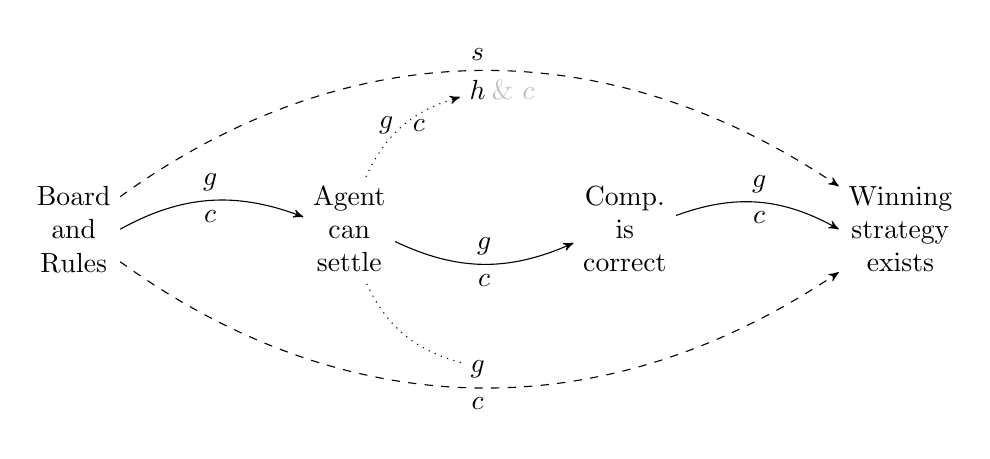
\begin{tikzpicture}[
  ->,
  >=stealth',
  % auto,
  node distance=0cm, every text node part/.style={align=center},
  ]

  \node (1) [] {Board \\ and \\ Rules};
  \node (2) [right of=1, xshift=3.5cm] {Agent \\ can \\ settle};
  \node (3) [right of=2, xshift=3.5cm] {Comp.\ \\ is \\ correct};
  \node (4) [right of=3, xshift=3.5cm] {Winning \\ strategy \\ exists};

  % \draw [->] (1.0) to [bend right=25] (2.180);
  % \draw [->] (2.0) to [bend left=25] (3.180);
  % \draw [->] (3.0) to [bend right=25] (4.180);

  \draw [->] (1.0) to [bend left=25] node[below] {\(c\)} node[above] {\(g\)} (2.165);
  \draw [->] (2.345) to [bend right=25] node[below] {\(c\)} node[above] {\(g\)} (3.195);
  \draw [->] (3.15) to [bend left=25] node[below] {\(c\)} node[above] {\(g\)} (4.180);

  \draw [dashed, ->] (1) to [bend left=35] node[below] (bSH) {\(h \)} node[above] (aSH) {\(s\)} (4);
  \node (x) [right of=bSH, xshift=.45cm, opacity=.25] {\(\&\mbox{ }c\)};
  % \draw [dotted, ->] (1) to [bend left=70] node[below] (bSC) {\(c\)} node[above] {\(s\)} (4);
  \draw [dashed, ->] (1) to [bend right=35] node[below] {\(c\)} node[above] (aGC) {\(g\)} (4);

  \draw [dotted, ->] (2) to [bend left=25] node[right] {\(c\)} node[left] {\(g\)} (bSH);
  % \draw [dotted, ->] (aSH) to [bend right=5] (bSC);
  \draw [dotted, -] (aGC) to [bend left=25] (2);
\end{tikzpicture}
\caption{Main relations}
\label{fig:dynamics}
\end{figure}

Roughly, there's a straightforward general categorical route to the agent's confidence that a winning strategy exists, but this also provides general categorical support for specific hypothetical support that a winning strategy exists.

\subsection{Notes}
\label{sec:notes}

So, what's important here is that there's a different \emph{type} of support available to the agent.
Namely, specific hypothetical (and likely categorical) support as opposed to general categorical support.

The role of the companion is to provide the agent with general categorical support that there is a winning strategy given the state of the board and the rules of chess.
And, after the agent establishes that there is general categorical support for a winning strategy given the state of the board and the rules of chess, it is this together with the agent's confidence that they are able to settle the question of whether there is a winning strategy which provides general categorical support for there being specific hypothetical support for the existence of a winning strategy given the board and the rules of chess.

The importance of the companion is, then, limited.
For example, there is potential for the companion to be providing testimony to the agent.
Yet, the scenario could be recast such that the companion is a somewhat limited computer program or any other instantiation of a random variable with the appropriate statistical properties (i.e.\ agreement with the agent's pattern of settling).
Of course, it may be the case that testimony is provided by the only plausible instantiations of random variables with the appropriate statistical properties, but even if testimony can be appealed to, I doubt that this resolves the puzzle.
For, even if the companion provides testimony that a winning strategy exists, it remains the case that the agent is confident that they are able to reason to the existence of a winning strategy independently of the companions (assumed) testimony.


\section{Inspector Morse and Sergeant Lewis}
\label{sec:second-case}

\begin{note}
  Below is a variation of the chess example that needs a little more work, but which I quite like.
  In short, Morse and Lewis are police officers who share the same powers of deduction and evidence.
  Lewis is a sergeant to Morse's role as inspector, but no longer wishes to enact Morse's commands.

  Lewis is the agent, Morse the companion, and Morse provides Lewis with the information that someone is a suspect given the evidence available to both Morse and Lewis.
  Lewis notices the suspect, and has no interest in approaching the person merely on the basis on Morse thinking that the person is a suspect.
  However, Lewis would approach the person if Lewis thought they were a suspect.
  Hence, given Morse's information about what Lewis could reason to, Lewis ends up approaching the person as a suspect.
\end{note}

Unlike Sherlock and Watson or Marple and a companion, Morse and Lewis are equally matched.\nolinebreak
\footnote{There is a lot that could be said about Morse and Lewis, but for background here a relevant detail is that the dynamic between Morse and Lewis is that of chance and privilege.}

Morse and Lewis have been working on a case together, share the same capacity to reason from evidence, and have examined the same evidence.
Lewis, as a sergeant, has been burdened with other tasks, and Morse is being recalcitrant.
In addition, Lewis has no interest in following Morse's orders.
The police stated is well staffed, and if Morse needs something to be done, and officer (other than Lewis) can be found.
However, Lewis will not refuse to perform a task if More thinks it needs to be done, Lewis' position is against performing a task that Lewis does not recognise as required by their role as a sergeant.

Lewis notices a message on their answer machine when returning home after work.
The message is from Morse who, given the lack of any new information, has been thinking about the case Morse and Lewis have been working on and thinks that it would be worthwhile for Person X to be brought in for questioning, but Morse does not explain why.
The unstated implication of Morse's message is that Lewis should bring Person X in for question tomorrow.
Lewis is confident that it would be worthwhile for Person X to be bought in for questioning, and that Lewis would arrive at this conclusion were they not so overburdened.
Still, bringing Person X in for questioning is a task that any officer could perform, so Lewis is under no pressure to seek Person X --- so tomorrow Lewis will explain to Morse that there are other officers at the police station.

Lewis' position, then, recognises that Morse thinks it is worthwhile for Person X to be brought in for questioning and that Lewis is in a position to recognise that it would be worthwhile for Person X to be bought in for questioning given the information available to Lewis.

The next morning, Lewis is on their way to work and notices Person X in the corner shop.
One the one hand, Lewis can radio in to the police station the location of a suspect that Morse would like to question.
One the other hand, Lewis is confident that they would have, were they to have thought more about the case, formed interest in questioning Person X themselves and Lewis recognises a requirement to themselves bring in for questioning suspects that they would like to question.
So, one the one hand Lewis' requirement is merely to inform the station that Person X has been sighted, while on the other hand Lewis' requirement would be to approach Person X themselves were they recognise the interest in questioning Person X.

Not much thinking is required, and Lewis approaches Person X, frustrated that they have not yet put together when they are interested in questioning Person X, but confident that they are not merely carrying out a task Morse thinks needs to be done.

\section{Middlemarch}
\label{sec:middlemarch}

\begin{note}
  I searched through Middlemarch for passages mentioning Pianos, and what follows is the only passage that seemed similar to the kind of cases I've been thinking about.

  However, I'm not sure that this quite works.
  For, it's not clear that Rosamond has any reason to think that Ladislaw's coming will require Lydgate to make plans to move to London.
  Instead, it seems as though Rosamond desires to go to London, but needs some cause for this to happen and Ladislaw's coming could be a cause, and (in a very Humean way) the constant conjunction of these two things in Rosamond's mind lead Rosamond to establish a relation of cause and effect that isn't supported by any particular reasons (though as Eliot notes, this kind of thing wouldn't be unique to Rosamond).

  Perhaps there's more to the story, though!
  It could be that Ladislaw is interested in Rosamond, Rosamond recognises this, but hasn't been able to identify the particular dynamic between Ladislaw and Lydgate which would lead Lydgate to make plans for London, but is confident given her general understanding of interpersonal relations that such a dynamic exists.
  Still, after reading through a few synopsis I'm not sure that this is the case\dots at the very least Rosamond here provides a nice contrast case.
\end{note}

\begin{quote}
  The next day Lydgate had to go to Brassing, and told Rosamond that he should be away until the evening.
  Of late she had never gone beyond her own house and garden, except to church, and once to see her papa, to whom she said,
  ``If Tertius goes away, you will help us to move, will you not, papa?
  I suppose we shall have very little money.
  I am sure I hope some one will help us.''
  And Mr.\ Vincy had said,
  ``Yes, child, I don't mind a hundred or two.
  I can see the end of that.''
  With these exceptions she had sat at home in languid melancholy and suspense, fixing her mind on Will Ladislaw's coming as the one point of hope and interest, and associating this with some new urgency on Lydgate to make immediate arrangements for leaving Middlemarch and going to London, till she felt assured that the coming would be a potent cause of the going, without at all seeing how.
  This way of establishing sequences is too common to be fairly regarded as a peculiar folly in Rosamond.
  And it is precisely this sort of sequence which causes the greatest shock when it is sundered: for to see how an effect may be produced is often to see possible missings and checks; but to see nothing except the desirable cause, and close upon it the desirable effect, rids us of doubt and makes our minds strongly intuitive.
  That was the process going on in poor Rosamond, while she arranged all objects around her with the same nicety as ever, only with more slowness---or sat down to the piano, meaning to play, and then desisting, yet lingering on the music stool with her white fingers suspended on the wooden front, and looking before her in dreamy ennui.
  Her melancholy had become so marked that Lydgate felt a strange timidity before it, as a perpetual silent reproach, and the strong man, mastered by his keen sensibilities towards this fair fragile creature whose life he seemed somehow to have bruised, shrank from her look, and sometimes started at her approach, fear of her and fear for her rushing in only the more forcibly after it had been momentarily expelled by exasperation.\linebreak
  \mbox{}\hfill\mbox{(Chapter LXXVII.)}
\end{quote}

\newpage

\section{Lord}
\label{sec:lord}

\begin{note}
  \citeauthor{Lord:2018aa}'s account of correctly responding to reasons seems a plausible account of what the agent fails to do in the chess scenario.
  For, the state of the board, the agent's grasp of the rules, and the agent's confidence that they can settle on whether there is a winning strategy suggest that the agent possesses reasons to believe that a winning strategy exists.

  However, as \citeauthor{Lord:2018aa} ties correctly responding to reasons to being rational, the agent in the chess example is irrational.
  Further, the agent is irrational even if they merely reason to general categorical support that there is a winning strategy given their confidence that they can settle on whether there is a winning strategy and the reliability of the companion, as it seems the agent possesses specific hypothetical (and categorical) reasons to believe that a winning strategy exists.
\end{note}

\begin{quote}
  You are \emph{ex ante} rational to believe that \emph{p} just in case \emph{p} is supported by sufficient justifiers.
  However, this isn't enough to have an \emph{ex post} rational belief that \emph{p}.
  In order to have an \emph{ex post} rational belief, there must be an appropriate connection between your belief and the justifiers of the belief.\nolinebreak
  \mbox{}\hfill\mbox{(\citeyear[70]{Lord:2018aa})}
\end{quote}

\begin{quote}
  [A] token \(\phi\)-ing is \emph{ex post} rational when
  \begin{enumerate*}[label=(\roman*), ref=\roman*.]
  \item one possesses normative reasons to \(\phi\) that are sufficiently weighty, and
  \item one \(\phi\)-s for those reasons.
  \end{enumerate*}
  \nolinebreak
  \mbox{}\hfill\mbox{(\citeyear[10]{Lord:2018aa})}
\end{quote}

\begin{quote}
  \textbf{Composite Possession}: What it is for agent \emph{A} to possess reason \emph{r} provided by fact \emph{f} to \(\phi\) is for
  \begin{enumerate*}[label=(\roman*), ref=\roman*.]
  \item\label{lord:posession:epistemic} \emph{A} to be in a position to know \emph{f} and
  \item\label{lord:posession:manifest} \emph{A} to be in a position to manifest knowledge about how to use \emph{r} to \(\phi\).
  \end{enumerate*}
  \nolinebreak
  \mbox{}\hfill\mbox{(\citeyear[123]{Lord:2018aa})}
\end{quote}

Strictly speaking, \citeauthor{Lord:2018aa} endorses `Possession', on the basis that condition \ref{lord:posession:epistemic} of `Composite Possession' is a background condition on possession.

\begin{quote}
  \textbf{Possession}: What it is for agent \emph{A} to possess reason \emph{r} to \(\phi\) provided by fact \emph{f} is for \emph{A} to be in a position to manifest knowledge about how to use \emph{r} to \(\phi\).
\end{quote}

\begin{quote}
  \textbf{Possession Enables Rational Routing}: If \emph{A} possesses \emph{r} as a sufficient reason to \(\phi\), then there is a route that \emph{A} can take to \emph{ex post} rational \(\phi\)-ing on the basis of \emph{r}.\nolinebreak
  \mbox{}\hfill\mbox{(\citeyear[100]{Lord:2018aa})}
\end{quote}

Key idea is that \citeauthor{Lord:2018aa} argues for is that the epistemic condition is insufficient as an account of reason possession and that the practical condition fills this gap.

This, seems right, to the extent that we focus on the agent's understanding of the board and the rules of chess it does not seem that the agent possess a reason for confidence that there is a winning strategy.
Instead, it is the combination (or the fulfilment of the background condition) of the agent's understanding of the board and the rules of chess \emph{with} the agent's confidence that the are in a position to use the board and their grasp of the rules of chess which suggests that the agent possesses a reason independently of the companion's answer for confidence that there is a winning strategy.

\begin{quote}
  \textbf{Normative}: \emph{A} \(\phi\)s for a normative reason \emph{r} just in case \emph{A} \(\phi\)s in virtue of the fact that \emph{r} is a normative reason to \(\phi\).
\end{quote}

\begin{quote}
  \textbf{Normative–Sustaining}: \emph{A} \(\phi\)s for a normative reason r if \emph{A} is disposed to revise her \(\phi\)-ing if r ceases to be a normative reason to \(\phi\).\nolinebreak
  \mbox{}\hfill\mbox{(\citeyear[138]{Lord:2018aa})}
\end{quote}

\begin{quote}
  \textbf{Normative–Production}: \emph{A} \(\phi\)s for a normative reason \emph{r} if \emph{A}'s \(\phi\)-ing is the manifestation of a disposition to \(\phi\) when the fact that constitutes \emph{r} is a normative reason to \(\phi\).\nolinebreak
  \mbox{}\hfill\mbox{(\citeyear[139]{Lord:2018aa})}
\end{quote}

\begin{quote}
  \textbf{Normative–Fleshed Out}: \emph{A} \(\phi\)s in virtue of the fact that \emph{r} is a normative reason to \(\phi\) just in case \emph{A}'s \(\phi\)-ing is produced or sustained by \emph{r} (in the ways specified by Normative–Sustaining and Normative–Production).\nolinebreak
  \mbox{}\hfill\mbox{(\citeyear[139]{Lord:2018aa})}
\end{quote}

\begin{quote}
  \textbf{Manifest}: What it is for \emph{A} to \(\phi\) for a normative reason \emph{r} is for \emph{A}'s \(\phi\)-ing to be a manifestation of \emph{A}'s knowledge about how to use \emph{r} as the reason it is to \(\phi\).\nolinebreak
  \mbox{}\hfill\mbox{(\citeyear[139]{Lord:2018aa})}
\end{quote}

\citeauthor{Lord:2018aa} takes `Manifest' to be an account of what it is to react for a normative reason.
\citeauthor{Lord:2018aa} argues, however, is that rationality is guarantee only if an agent's reactions are supported by sufficiently strong normative reasons.
(\citeyear[141]{Lord:2018aa})

\citeauthor{Lord:2018aa} provides the following account of reacting to a sufficient normative reason.

\begin{quote}
  \textbf{Sufficient Normative}: \emph{A} \(\phi\)s for a sufficient normative reason \emph{r} just in case \emph{A} \(\phi\)s in virtue of the fact that \emph{r} is a sufficient normative reason to \(\phi\).\nolinebreak
  \mbox{}\hfill\mbox{(\citeyear[142]{Lord:2018aa})}
\end{quote}

The key here is the `in virtue of' relation, understood through two requirements of an agent's dispositions.

\begin{quote}
  \textbf{Sufficient Normative–Sustaining}: \emph{A} \(\phi\)-s for a sufficient normative reason \emph{r} if \emph{A} is disposed to cease \(\phi\)-ing when \emph{r} ceases to be a sufficient normative reason to \(\phi\).\nolinebreak
  \mbox{}\hfill\mbox{(\citeyear[142]{Lord:2018aa})}
\end{quote}

\begin{quote}
  \textbf{Sufficient Normative–Production}: \emph{A} \(\phi\)s for a sufficient normative reason \emph{r} if \emph{A}'s \(\phi\)-ing is the manifestation of a disposition to \(\phi\) when the fact that constitutes \emph{r} is a sufficient normative reason to \(\phi\).\nolinebreak
  \mbox{}\hfill\mbox{(\citeyear[142]{Lord:2018aa})}
\end{quote}

\citeauthor{Lord:2018aa} suggests that the disjunction of sustaining and manifesting forms a necessary and sufficient condition fir reacting for a sufficient normative reason.

\begin{quote}
  \textbf{Sufficient Normative–Fleshed Out}: \emph{A} \(\phi\)s for a sufficient normative reason \emph{r} just in case \emph{A}'s \(\phi\)-ing is sustained or produced by the fact that \emph{r} is a sufficient normative reason to \(\phi\).\nolinebreak
  \mbox{}\hfill\mbox{(\citeyear[143]{Lord:2018aa})}
\end{quote}

For \citeauthor{Lord:2018aa} reacting to sufficient normative reasons is understood in terms of know-how, leading to:

\begin{quote}
  \textbf{Manifest Sufficient}: What it is for \emph{A} to \(\phi\) for a sufficient normative reason to \(\phi\) is for \emph{A} to manifest knowledge about how to use \emph{r} as the sufficient reason it is to \(\phi\).\nolinebreak
  \mbox{}\hfill\mbox{(\citeyear[143]{Lord:2018aa})}
\end{quote}

This, then completes \citeauthor{Lord:2018aa}'s account of \emph{ex post} rationality.

\begin{quote}
  \textbf{Correctly Responding}: What it is for \emph{A}'s \(\phi\)-ing to be \emph{ex post} rational is for \emph{A} to possess sufficient reason \emph{S} to \(\phi\) and for \emph{A}'s \(\phi\)-ing to be a manifestation of knowledge about how to use \emph{S} as sufficient reason to \(\phi\).\nolinebreak
  \mbox{}\hfill\mbox{(\citeyear[143]{Lord:2018aa})}
\end{quote}

So, in \citeauthor{Lord:2018aa}'s terminology it seems the agent is in a position to be \emph{ex post} rational confidence that there is a winning strategy given the board and the agent's grasp of the rules of chess.
However, the agent does not manifest the appropriate knowledge of how to use the board and the rules of chess to demonstrate the existence of a winning strategy, and hence the agent is not \emph{ex post} rational.

This seems plausible to me.
Of course, there are details that matter, but in broad strokes it is the agent's failure to reason from the board and their grasp of the rules which is striking, and if the agent were to respond to their possessed reasons by reasoning to a winning strategy, then there doesn't seem to be anything particularly interesting about the scenario.
Still, if the agent does not correctly respond to the possessed reasons for a winning strategy, then the agent is not rational on \citeauthor{Lord:2018aa} account, and this is somewhat unsatisfying.



A further question is whether, on \citeauthor{Lord:2018aa}'s account, there is pressure for the agent to believe that there is a winning strategy based on their confidence that they can settle on an answer to whether there is a winning strategy.
\citeauthor{Lord:2018aa} notes three relevant principles.

\begin{quote}
  \textbf{Belief Schema}: If the set of reasons you possess decisively supports \emph{p}, then you are rationally required to believe that \emph{p}.\nolinebreak
  \mbox{}\hfill\mbox{(\citeyear[28]{Lord:2018aa})}
\end{quote}

\begin{quote}
  \textbf{Closure Transmission}: If the reasons you possess decisively support \emph{p} and the reasons you possess decisively support if \emph{p} then \emph{q}, then the reasons you possess decisively support \emph{q}.
\end{quote}

\begin{quote}
  \textbf{Reasons-Coherence, Closure}: If you are closure incoherent, then you are not correctly responding to all of the reasons you possess.
\end{quote}

\citeauthor{Lord:2018aa}'s account of possession limits the scope of Closure/Coherence, as the agent must be able to manifest knowledge about how to use the reason.
This means that it doesn't apply to cases such as the preface paradox, as the condition does not require coherence between arbitrary collections of attitudes.
Still, this does not exclude the chess case, as plausibly it is the case that the reasons the agent possesses do decisively support believing that there is a winning strategy.

The relevant problem is that the agent should recognise that they do not satisfy coherence by `merely' having the required attitude.
Coherence, on \citeauthor{Lord:2018aa}'s view, is a result of correct responsiveness, and so does not seem as though the agent should worry about closure if they recognise that they have not correctly responded to the reasons in their possession.

So, it does not seem that, on \citeauthor{Lord:2018aa}'s account the agent is under pressure to believe that there is a winning strategy given the state of the board and the rules of chess, as the relevant form of irrationality is the failure of the agent to correctly respond to the reasons that they possess.

In part, this can be seen by \citeauthor{Lord:2018aa}'s argument for Reasons-Coherence, Closure.

\begin{quote}
  Reasons-Coherence, Closure is true because it will either be true that you possess decisive reason to believe \emph{p}, decisive reason to believe if \emph{p} then \emph{q} and thus by Closure Transmission possess decisive reason to believe \emph{q}, or you won't.
  If you do possess decisive reason to believe \emph{p}, decisive reason to believe if \emph{p} then \emph{q}, then you'll possess decisive reason to believe \emph{q}, and thus you are irrational when closure incoherent because you don't believe \emph{q}.
  If you lack decisive reason to believe \emph{p} or lack decisive reason to believe if \emph{p} then \emph{q}, then you will be irrational when closure incoherent because you hold one of those beliefs and you are rationally required not to.
  Either way, you will be irrational when closure incoherent.
\end{quote}

Here, \citeauthor{Lord:2018aa} identifies the irrationality of being closure incoherent in terms of failing to correctly respond to possessed reasons.
Therefore, as the agent has not (yet, at least) responding to their possessed reasons in the chess scenario, the agent is irrational, and moreover there is no clear explanation for why the agent would (incorrectly) respond to their possessed reasons as there is no route to rationality other than by correctly responding to their reasons.

% \newpage

% \section{Awake at night}
% \label{sec:awake-at-night}

% Heck, there's something about these kinds of cases that keeps me up at night.
% Because these kinds of parallels suggest that I should be confident that I have some problematic attitudes.
% The contrast is that I don't know what the result of reasoning from these attitudes would be.
% At least these aren't genuine reasons, though.

\newpage

\printbibliography


\end{document}
